 \section{Prototype work}
For this sprint we created a few new prototypes aswell as refactoring some of the older designs. 
Most of the new prototypes created were based on the feedback we got from the usability test we held in sprint 3 (see \autoref{usability-test-sprint-3})

\subsection{Choiceboard}

\begin{figure}[H]
    \begin{subfigure}{0.5\textwidth}
    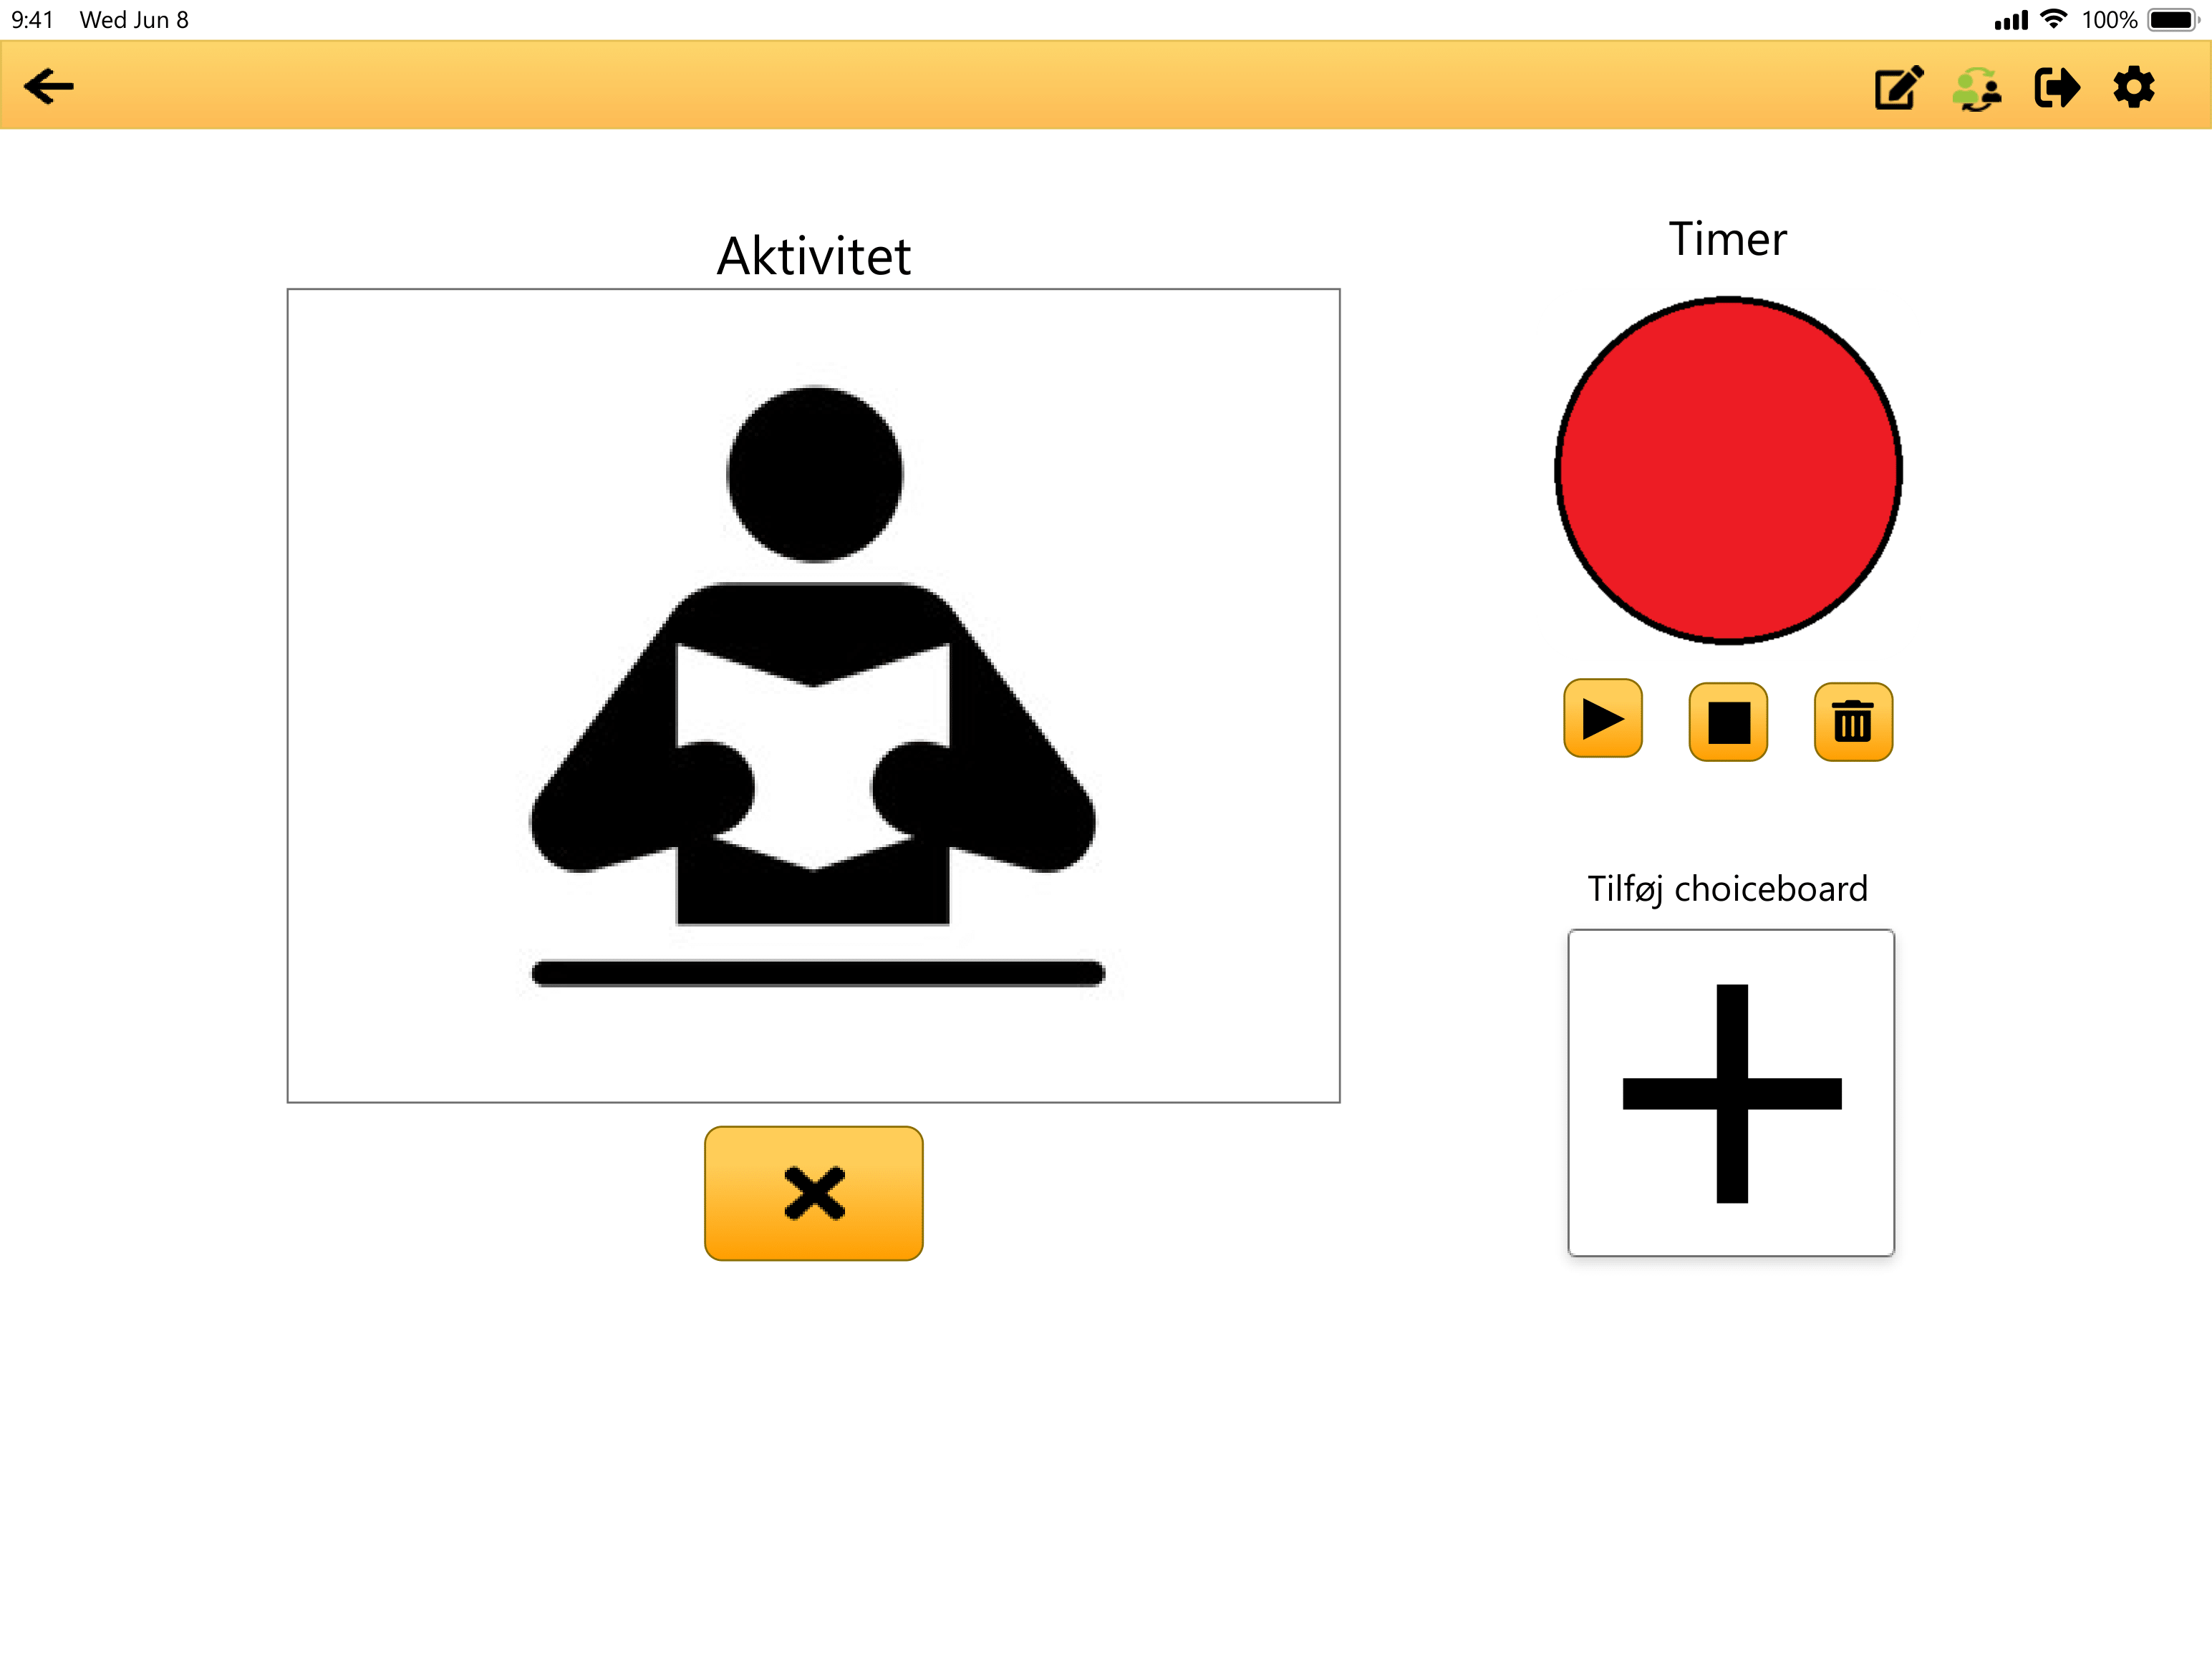
\includegraphics[width=1\linewidth, height=5cm]{choiceboard_1.png}
    \caption{Adding choiceboard to an activity}
    \label{subfig:choiceboard_1}
    \end{subfigure}
    \begin{subfigure}{0.5\textwidth}
    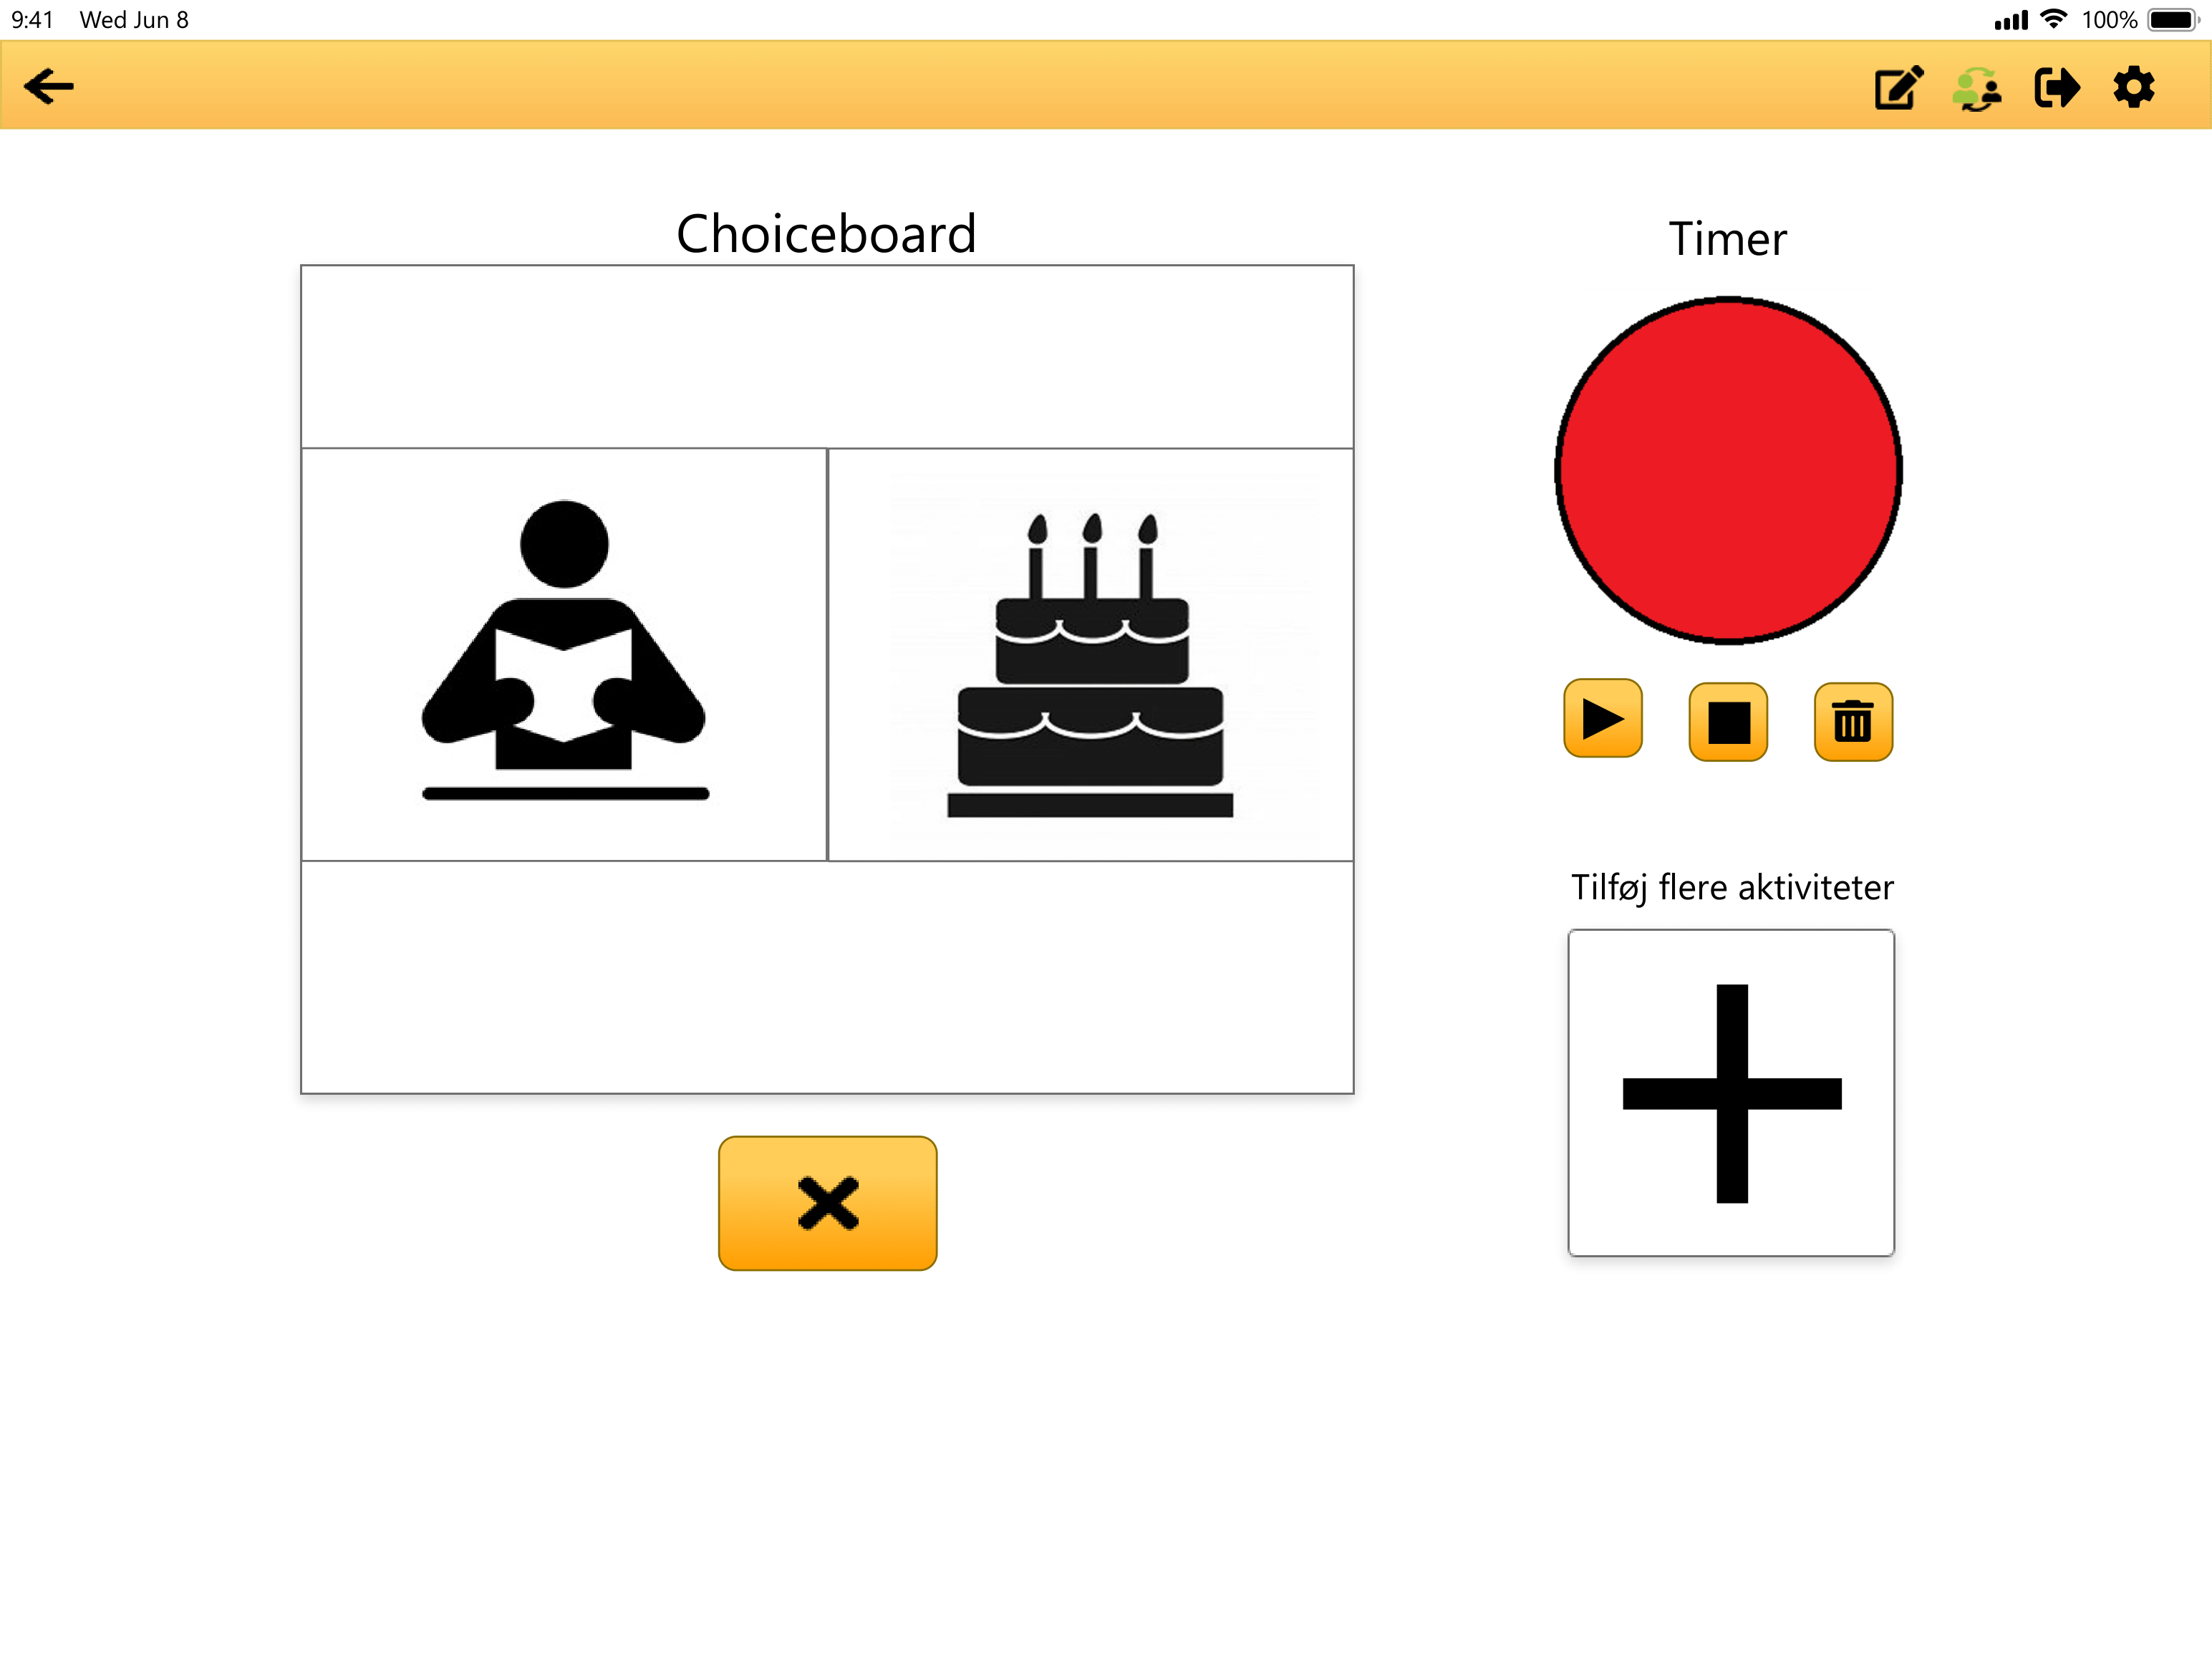
\includegraphics[width=1\linewidth, height=5cm]{choiceboard_2.png}
    \caption{Adding more activities to a choiceboard}
    \label{subfig:choiceboard_2}
    \end{subfigure} 
    \caption{}
    \label{fig:choiceboard_1}
\end{figure}

\begin{figure}[H]
    \begin{subfigure}{0.5\textwidth}
    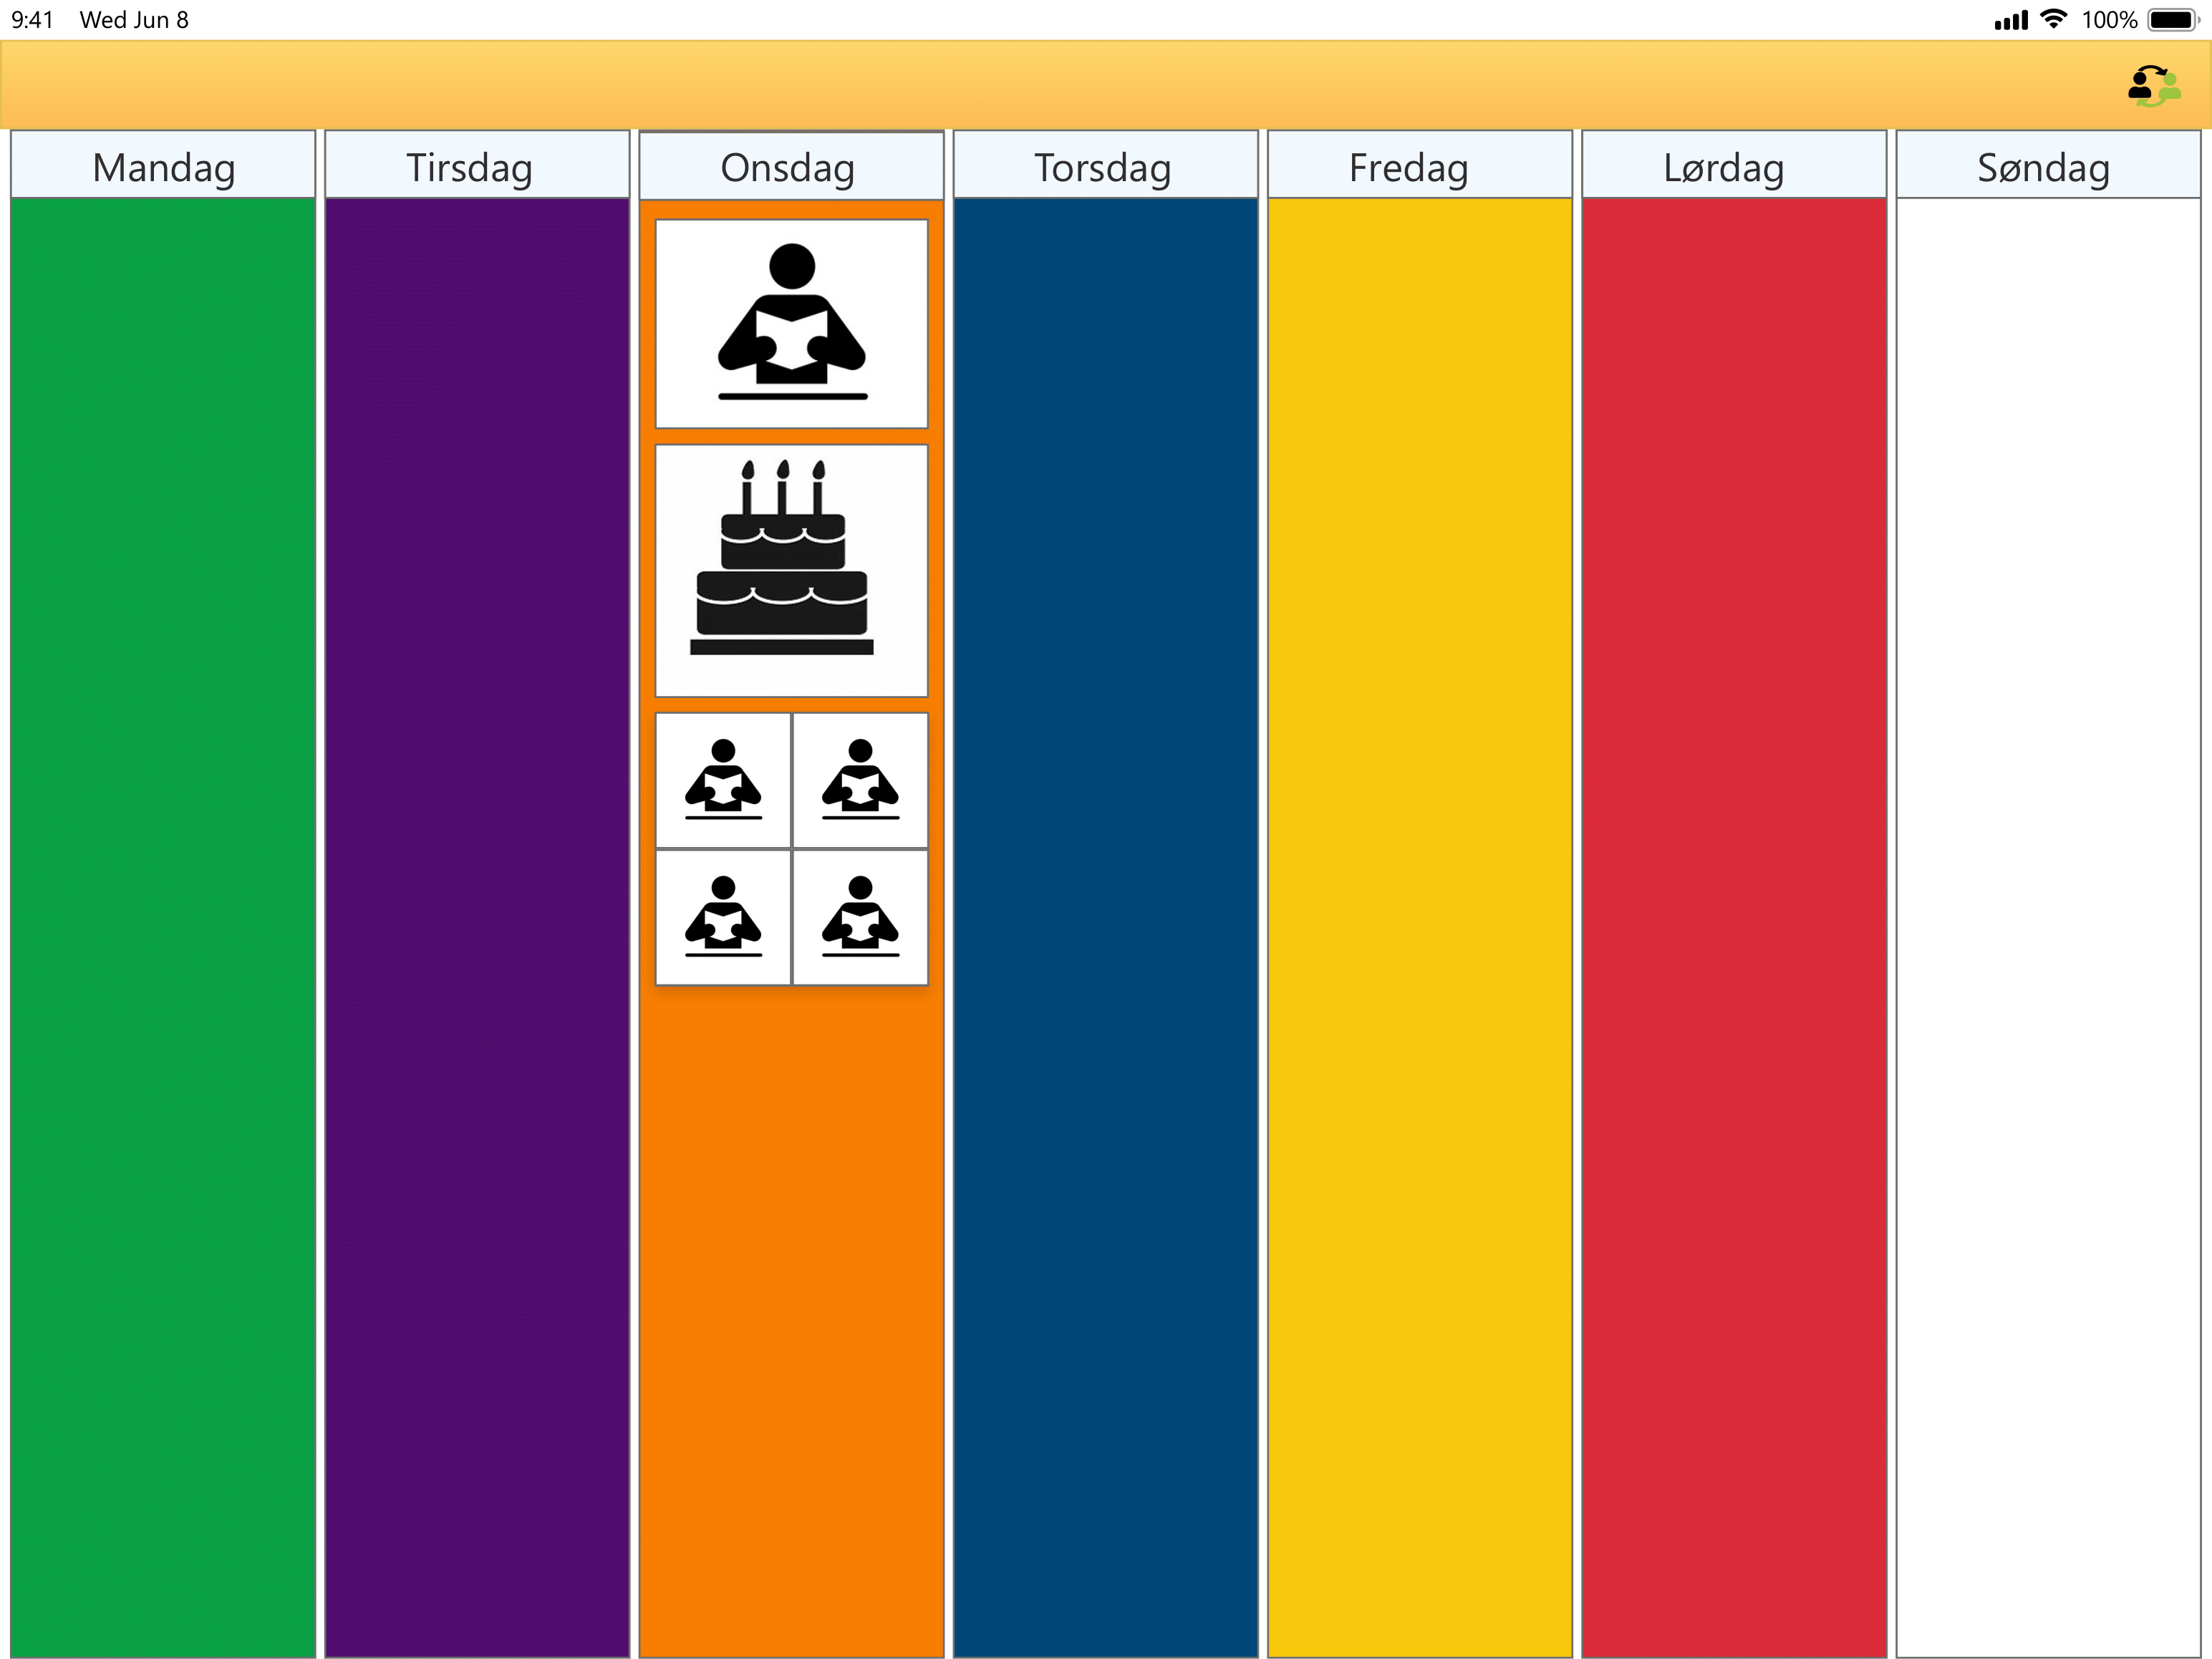
\includegraphics[width=1\linewidth, height=5cm]{choiceboard_5.png}
    \caption{Choiceboard as seen on the citizens view}
    \label{subfig:choiceboard_5}
    \end{subfigure}
    \begin{subfigure}{0.5\textwidth}
        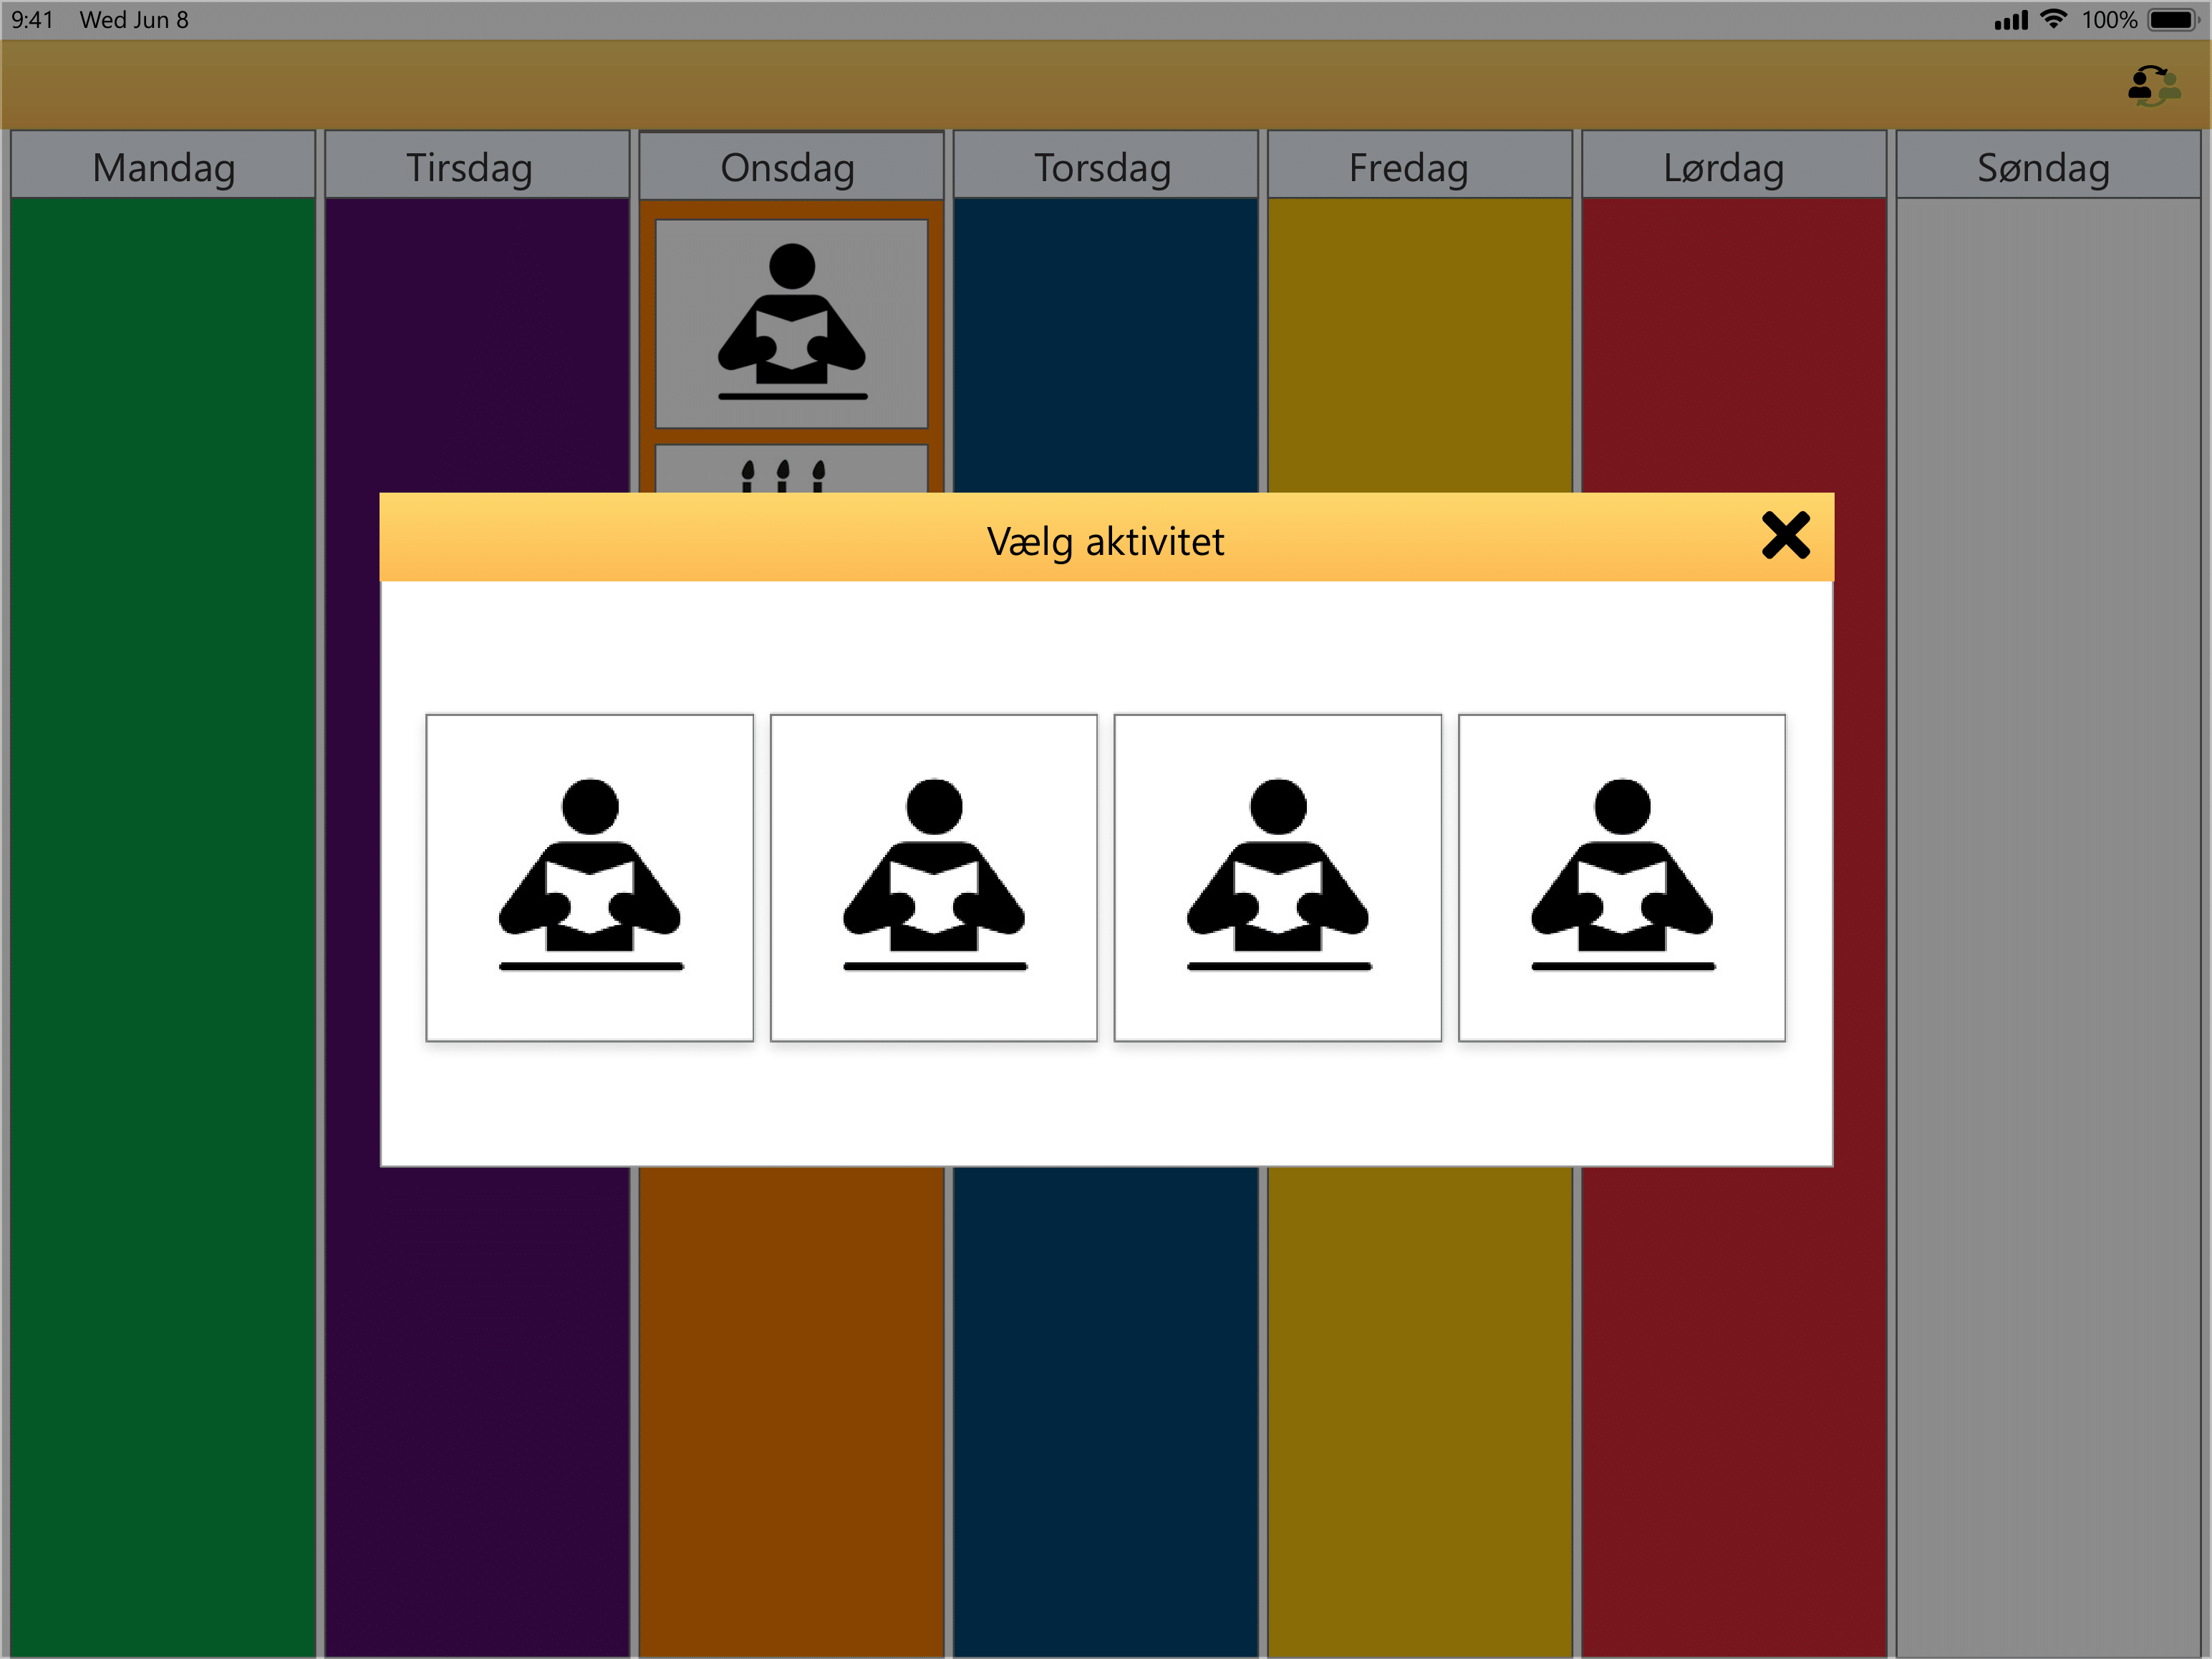
\includegraphics[width=1\linewidth, height=5cm]{choiceboard_6.png}
    \caption{Citizen chooses an activity from choiceboard}
    \label{subfig:choiceboard_6}
    \end{subfigure} 
    \caption{}
    \label{fig:choiceboard_2}
\end{figure}

\subsection{Lock timer}

\begin{figure}[H]
    \begin{subfigure}{0.5\textwidth}
    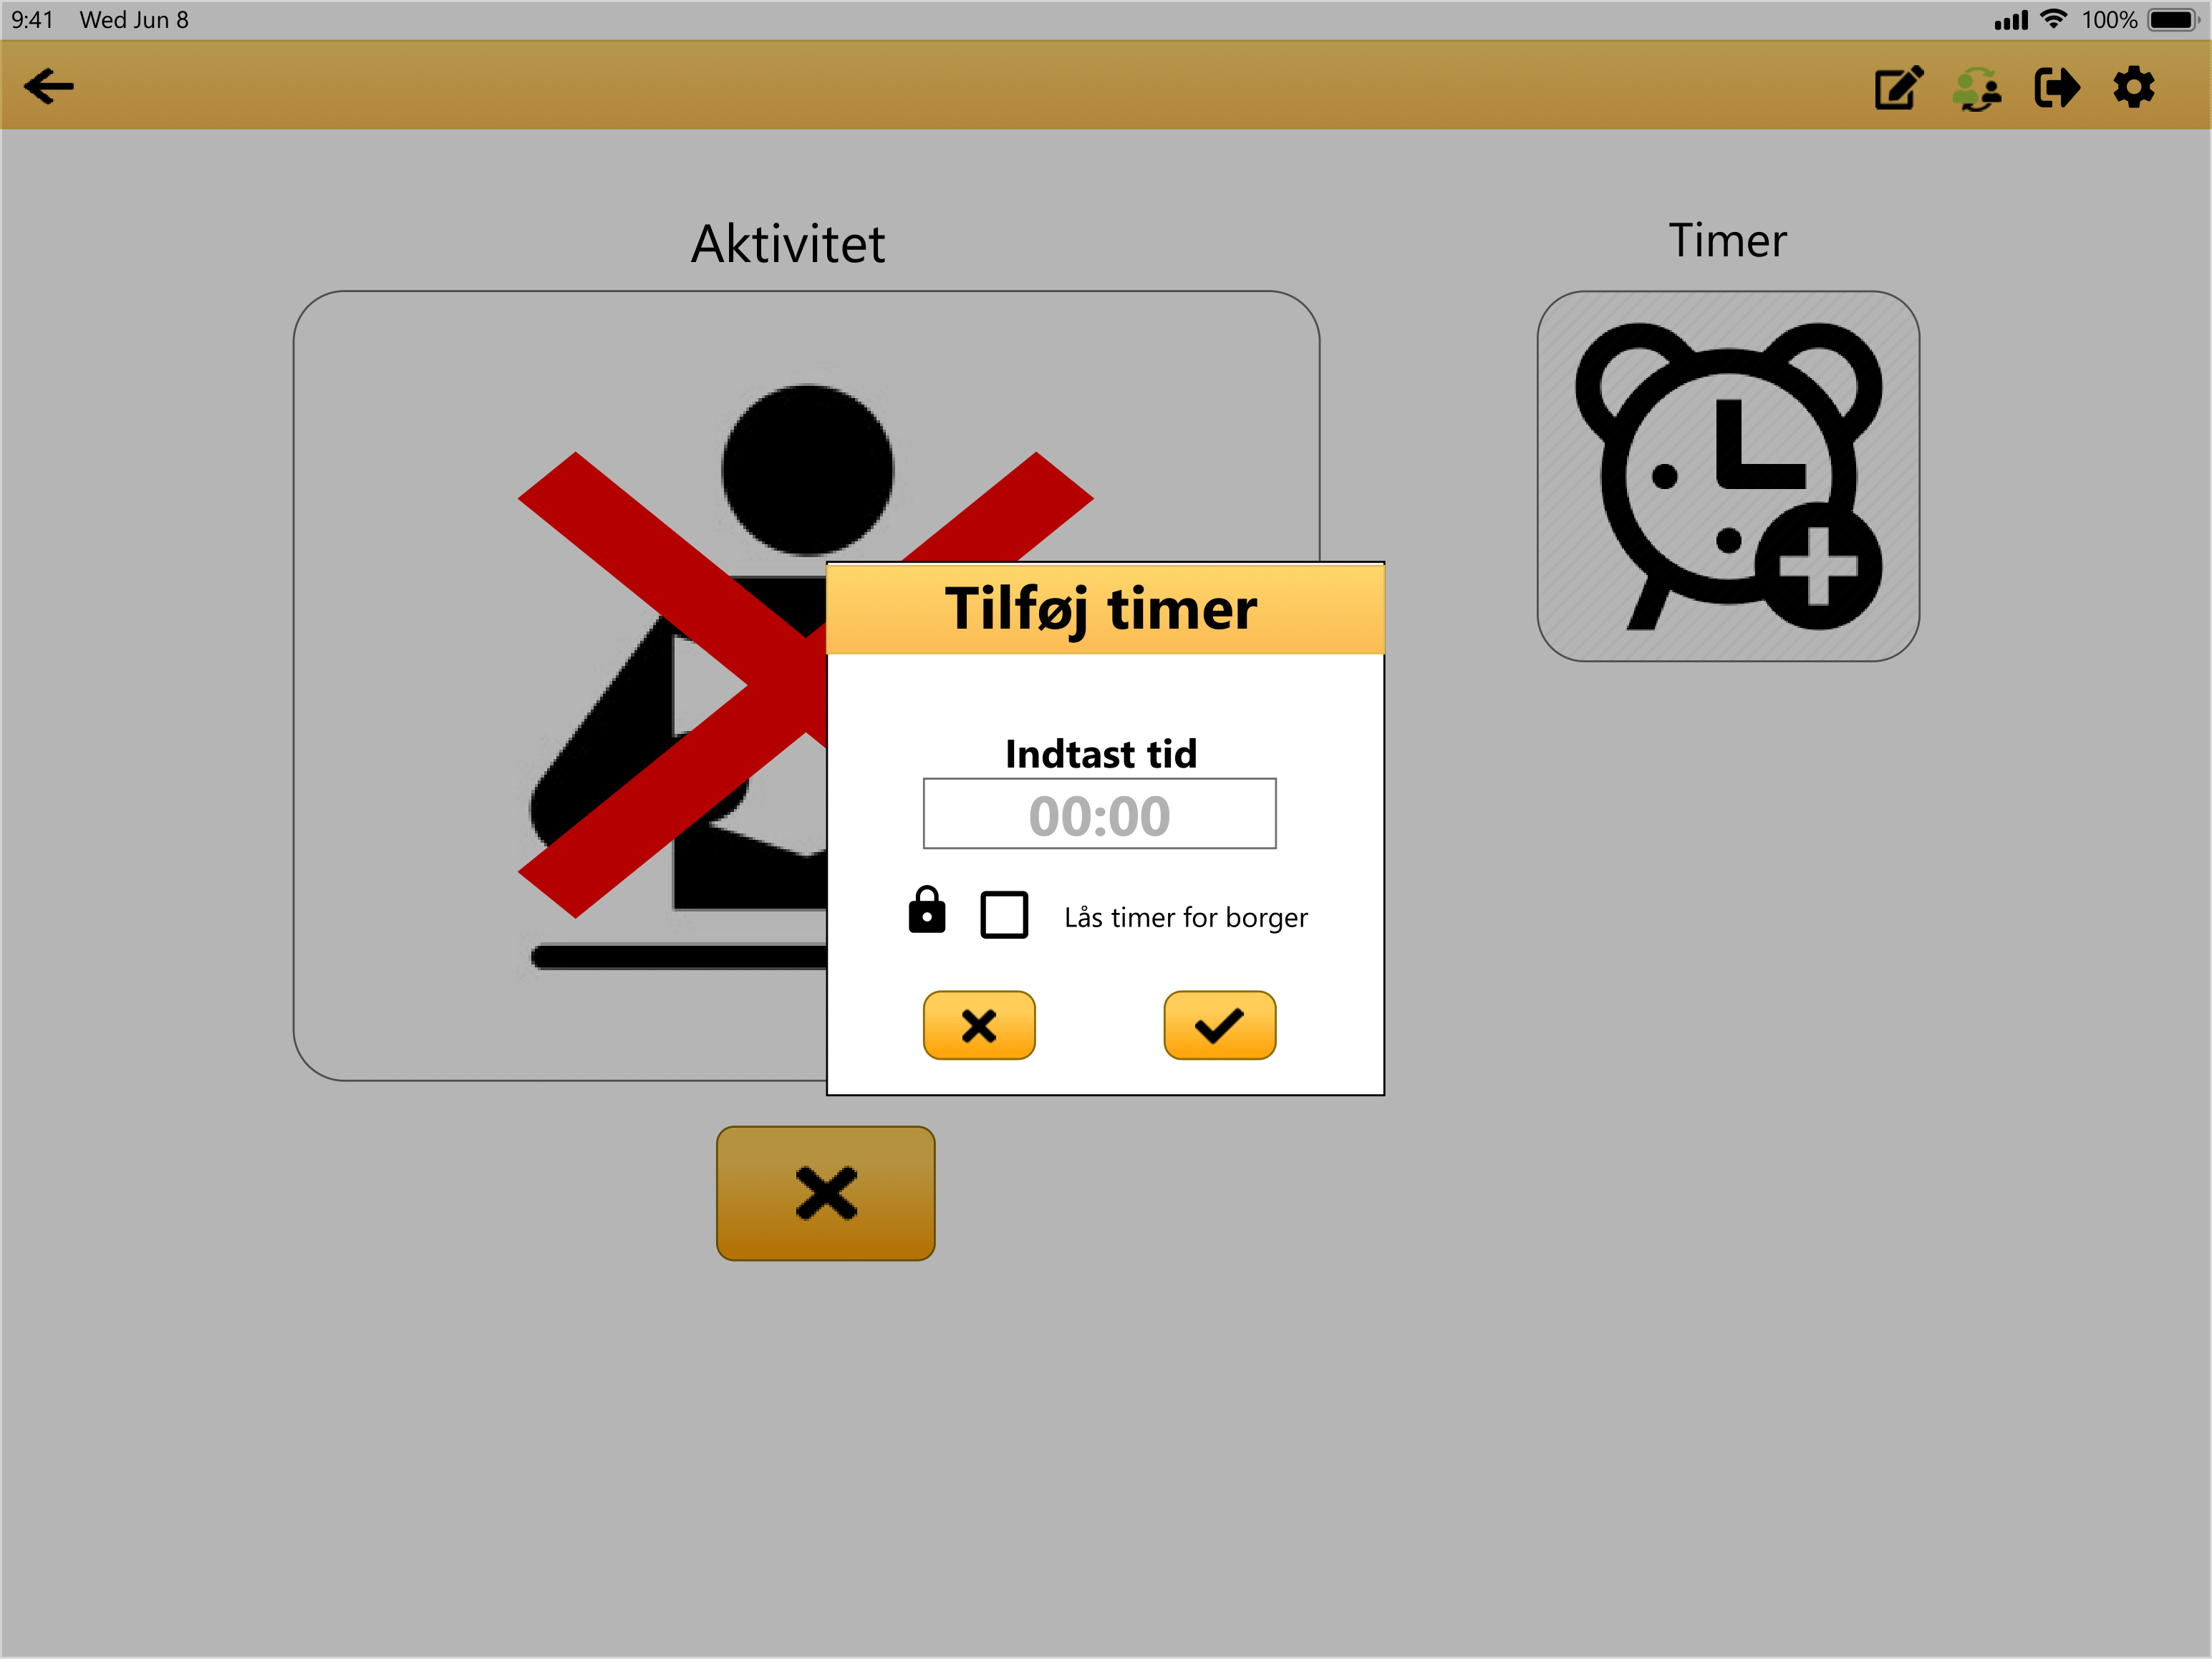
\includegraphics[width=1\linewidth, height=5cm]{lock_timer_1.png}
    \caption{Checkmark to lock timer}
    \label{subfig:lock_timer_1}
    \end{subfigure}
    \begin{subfigure}{0.5\textwidth}
        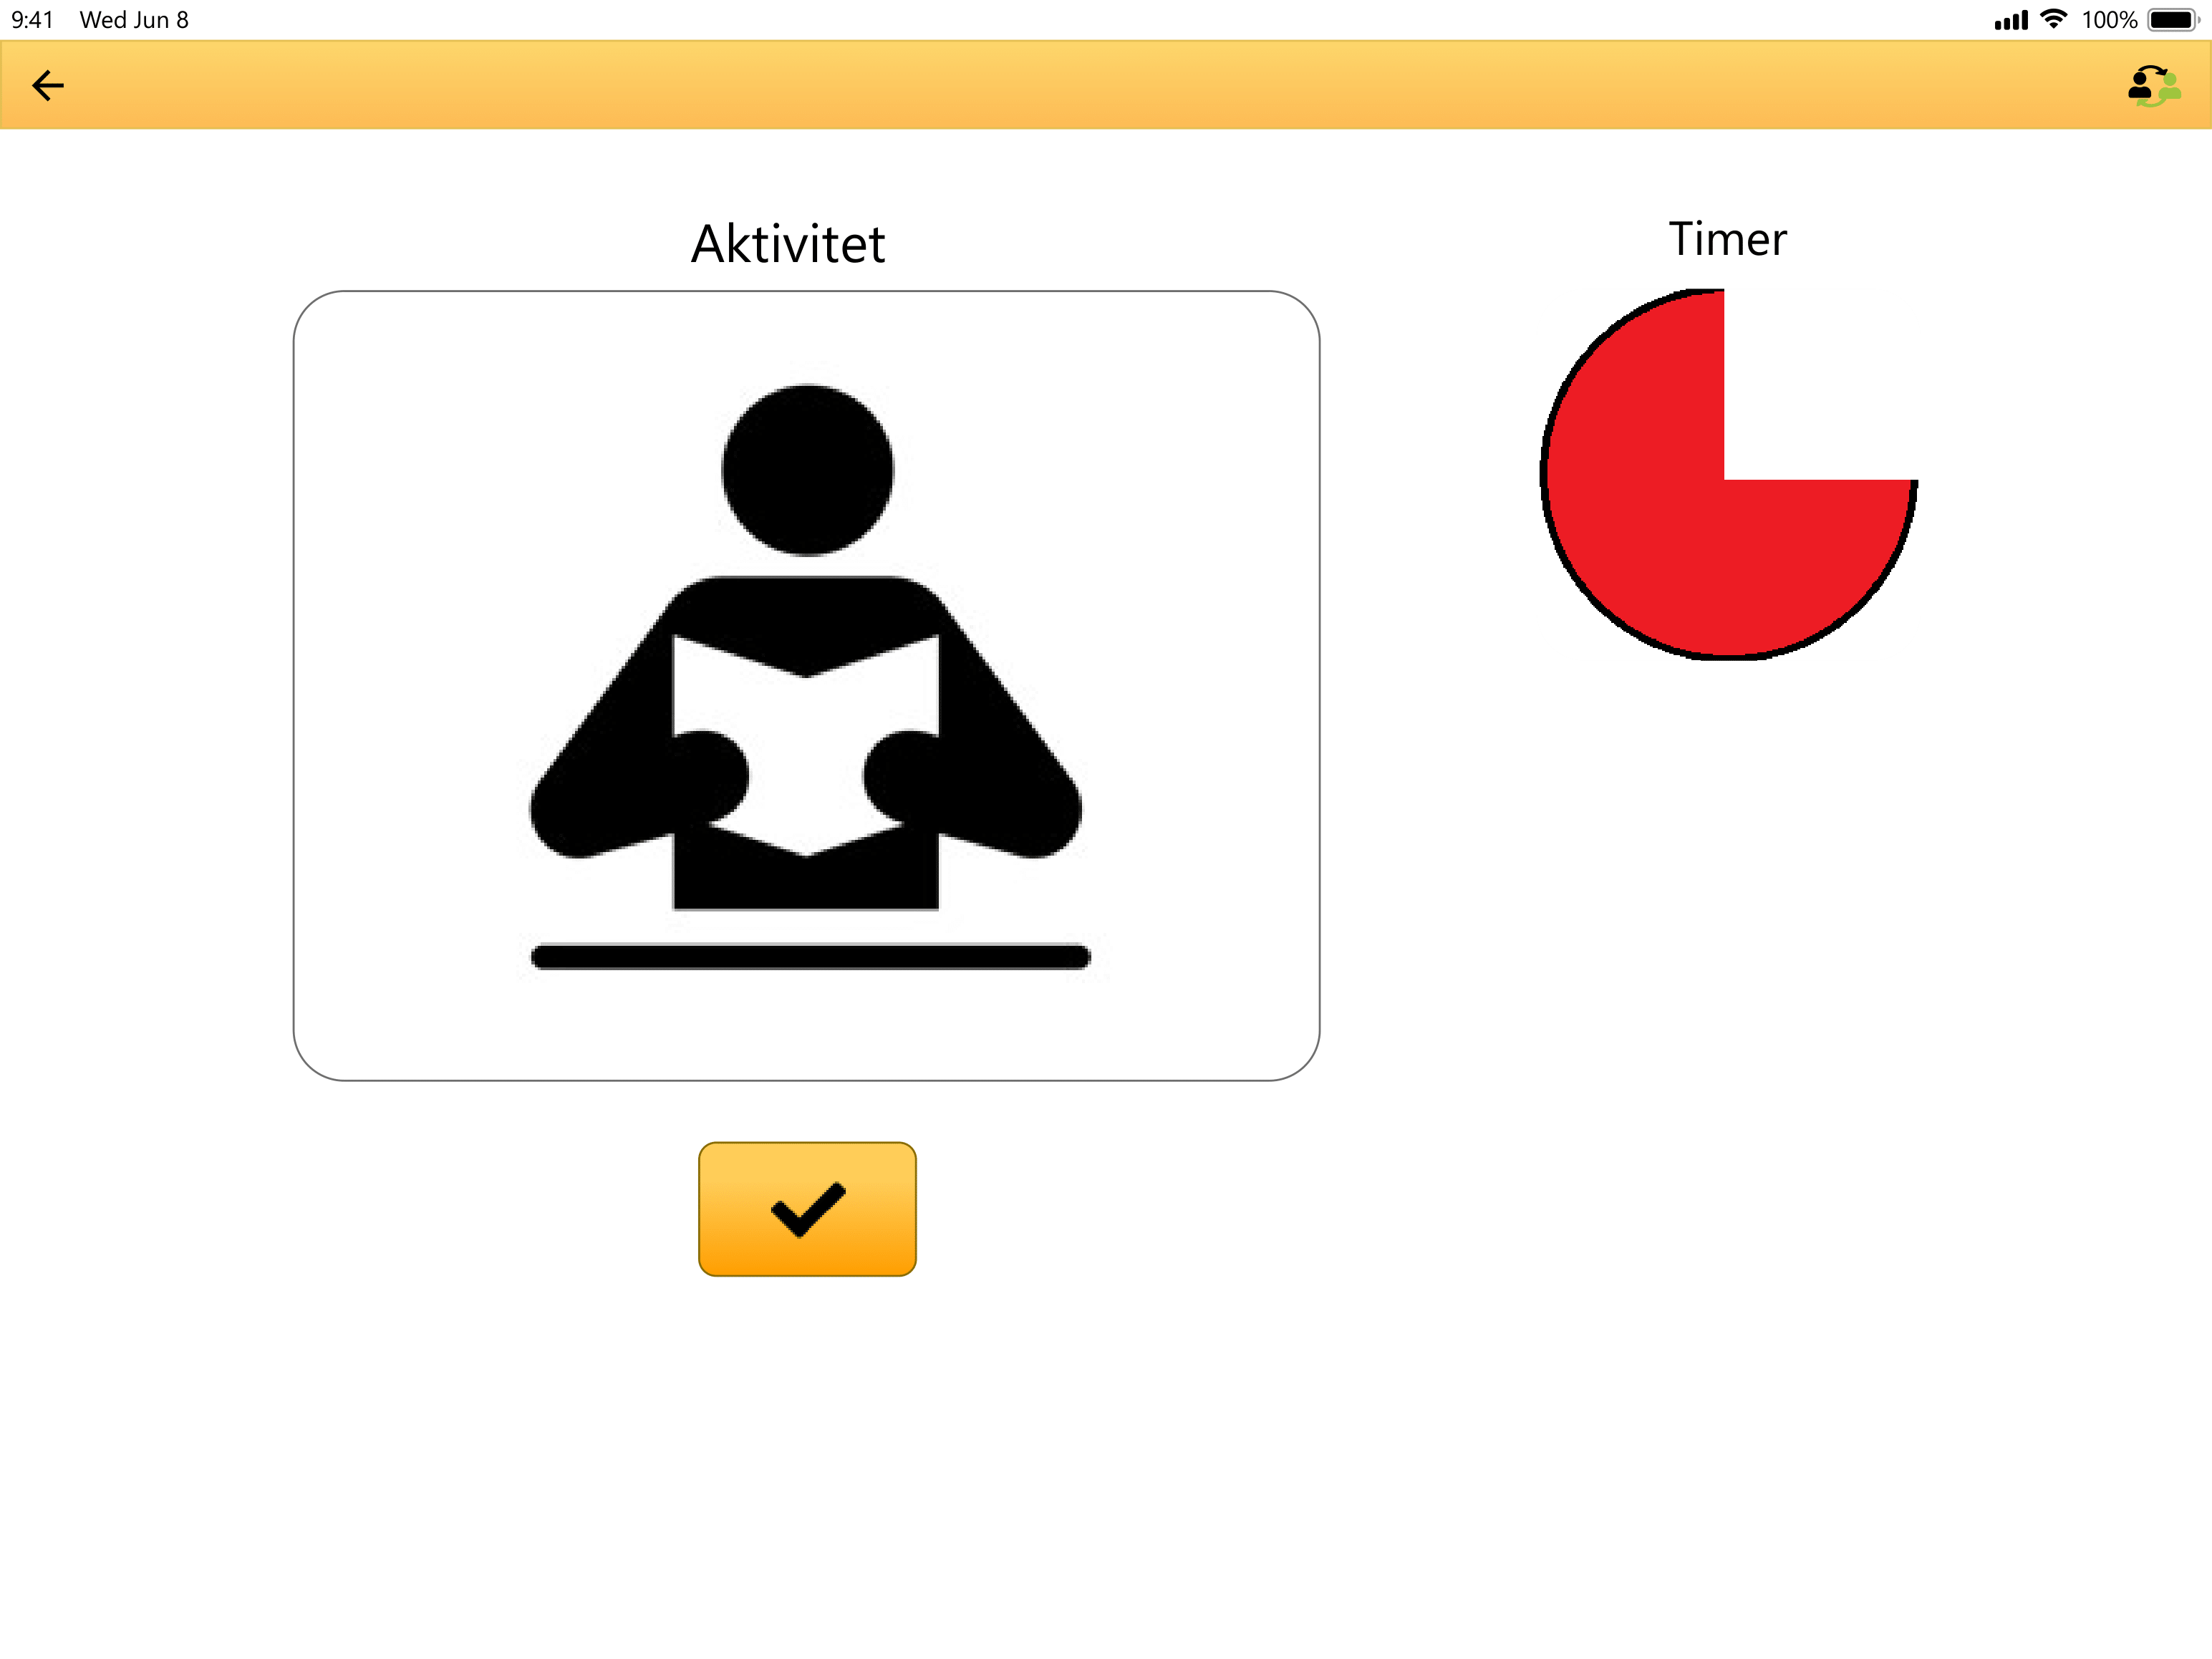
\includegraphics[width=1\linewidth, height=5cm]{lock_timer_3.png}
    \caption{No pause button for citizen on the timer}
    \label{subfig:lock_timer_3}
    \end{subfigure} 
    \caption{}
    \label{fig:lock_timer}
\end{figure}

\subsection{Drag and drop activities}

\begin{figure}[H]
    \begin{subfigure}{0.5\textwidth}
    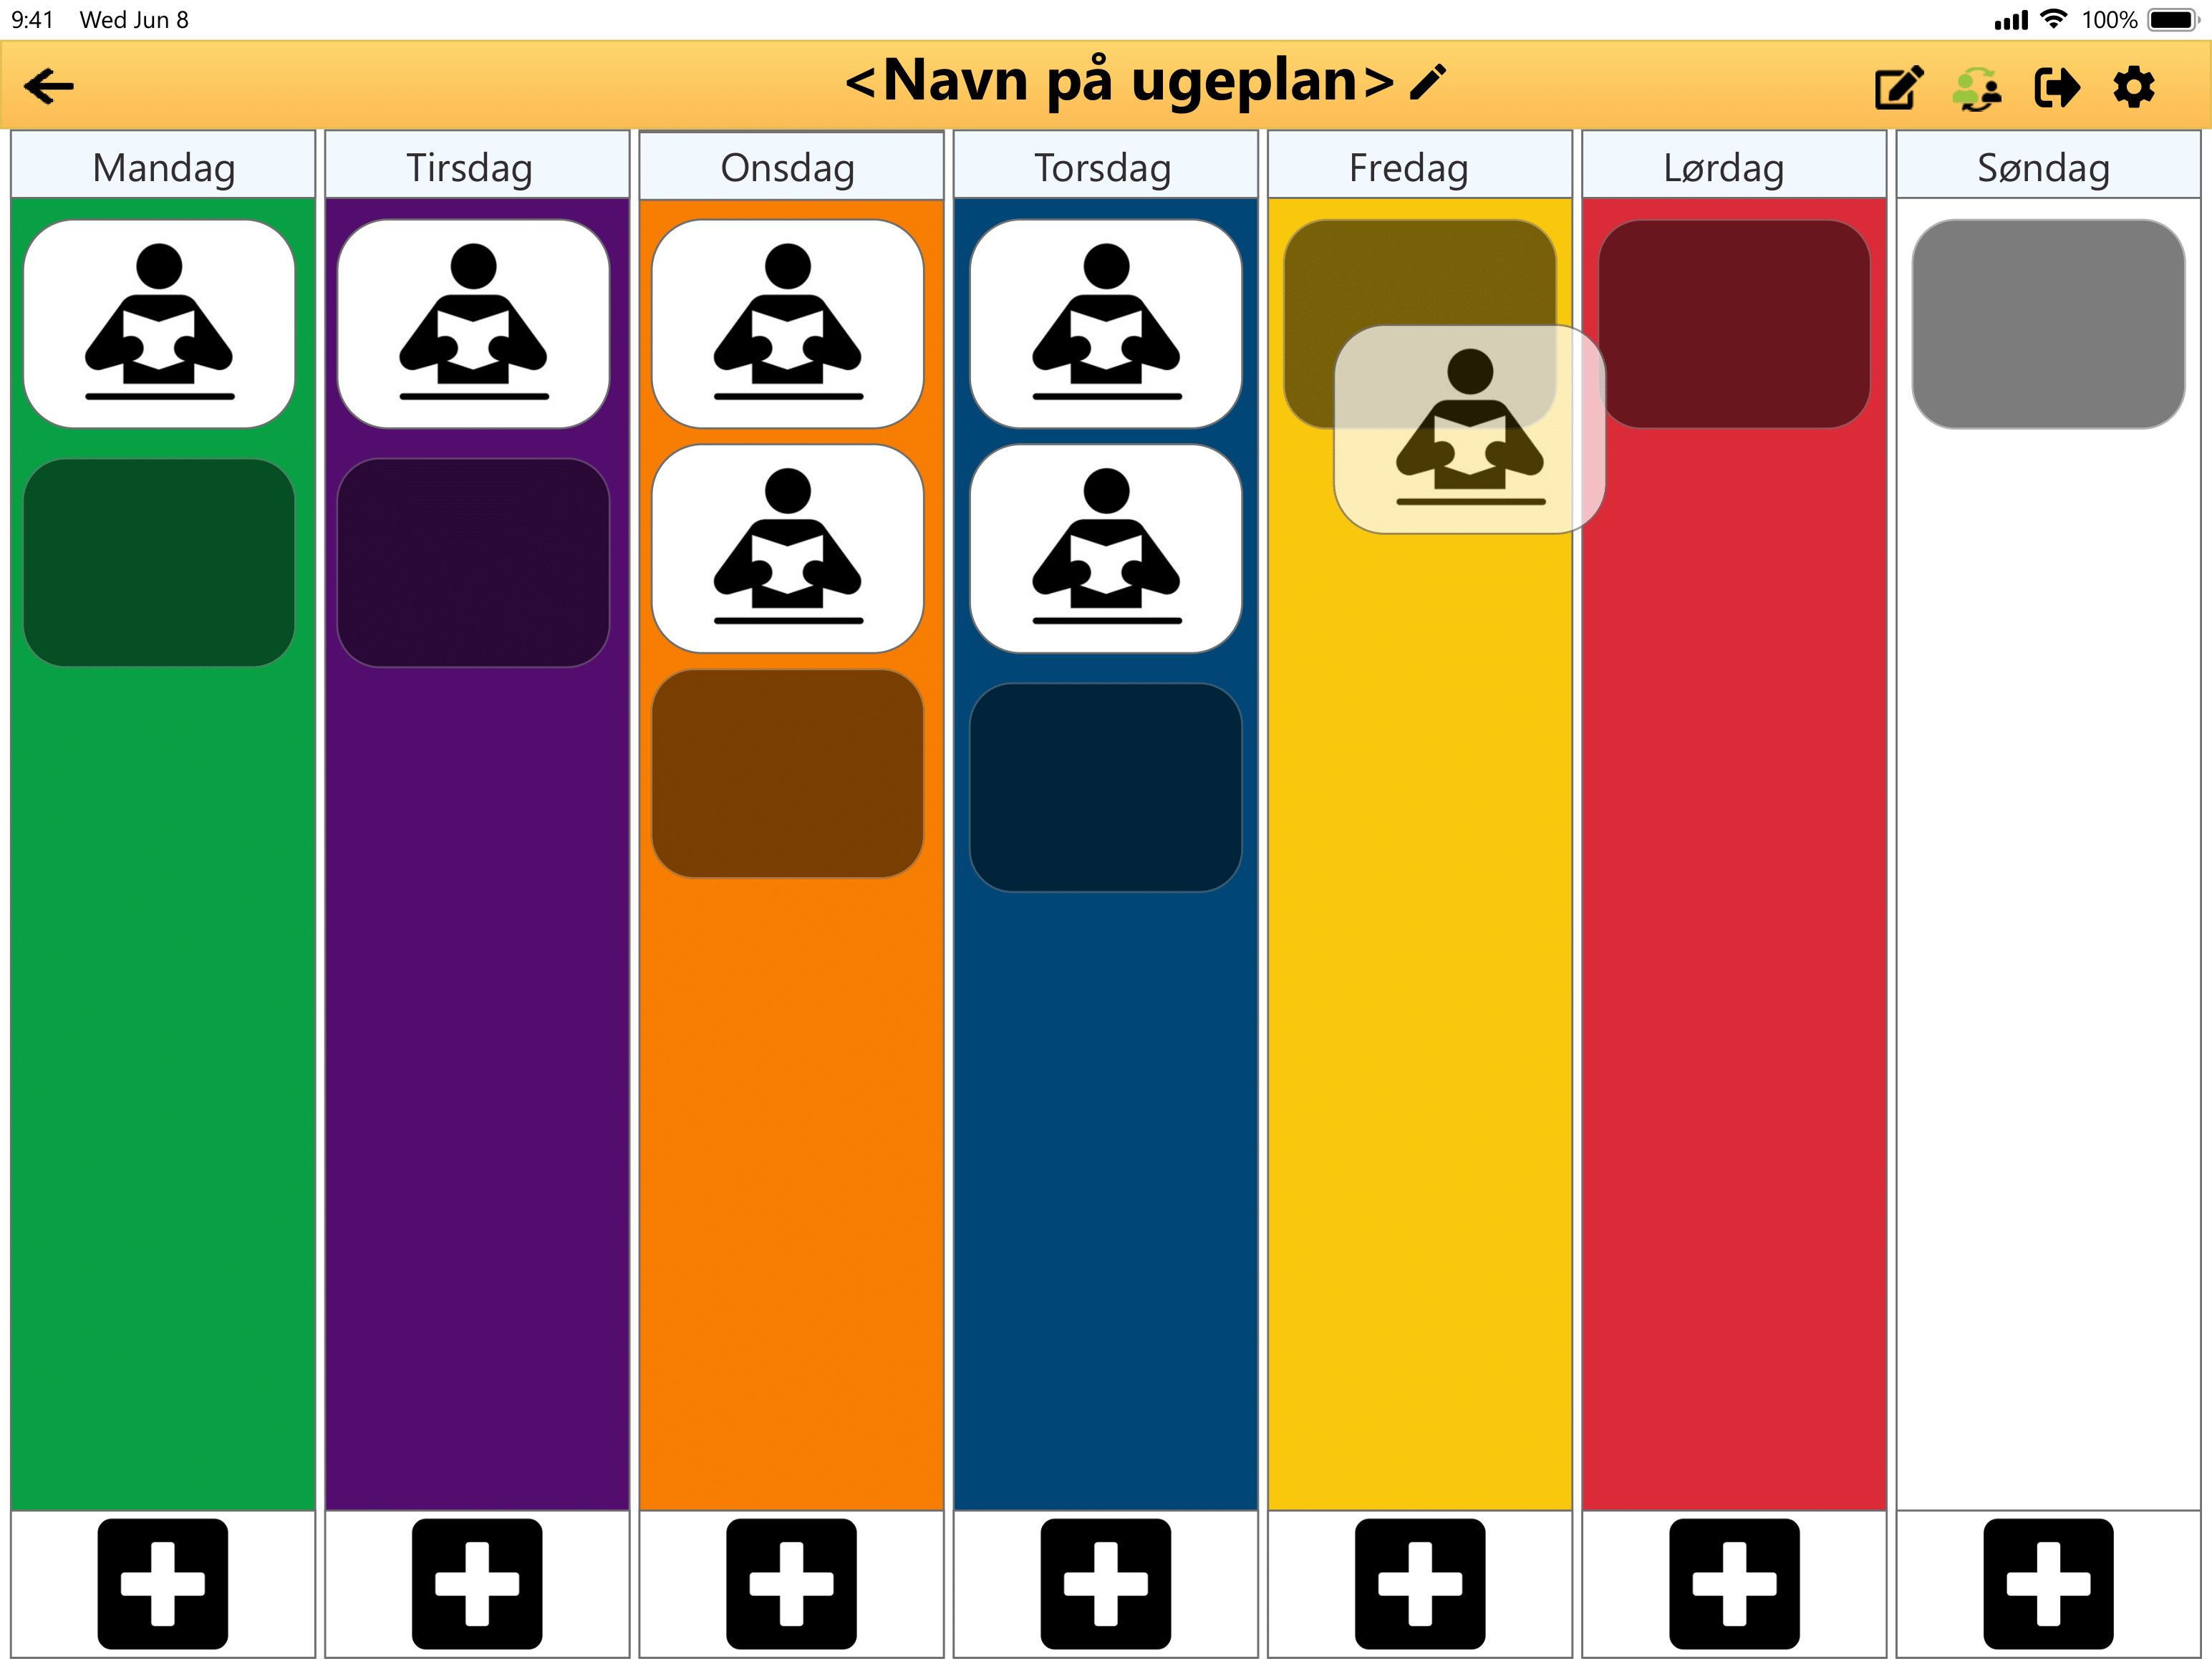
\includegraphics[width=1\linewidth, height=5cm]{drag_n_drop_2.png}
    \caption{Dragging an activity}
    \label{subfig:drag_n_drop_2}
    \end{subfigure}
    \begin{subfigure}{0.5\textwidth}
        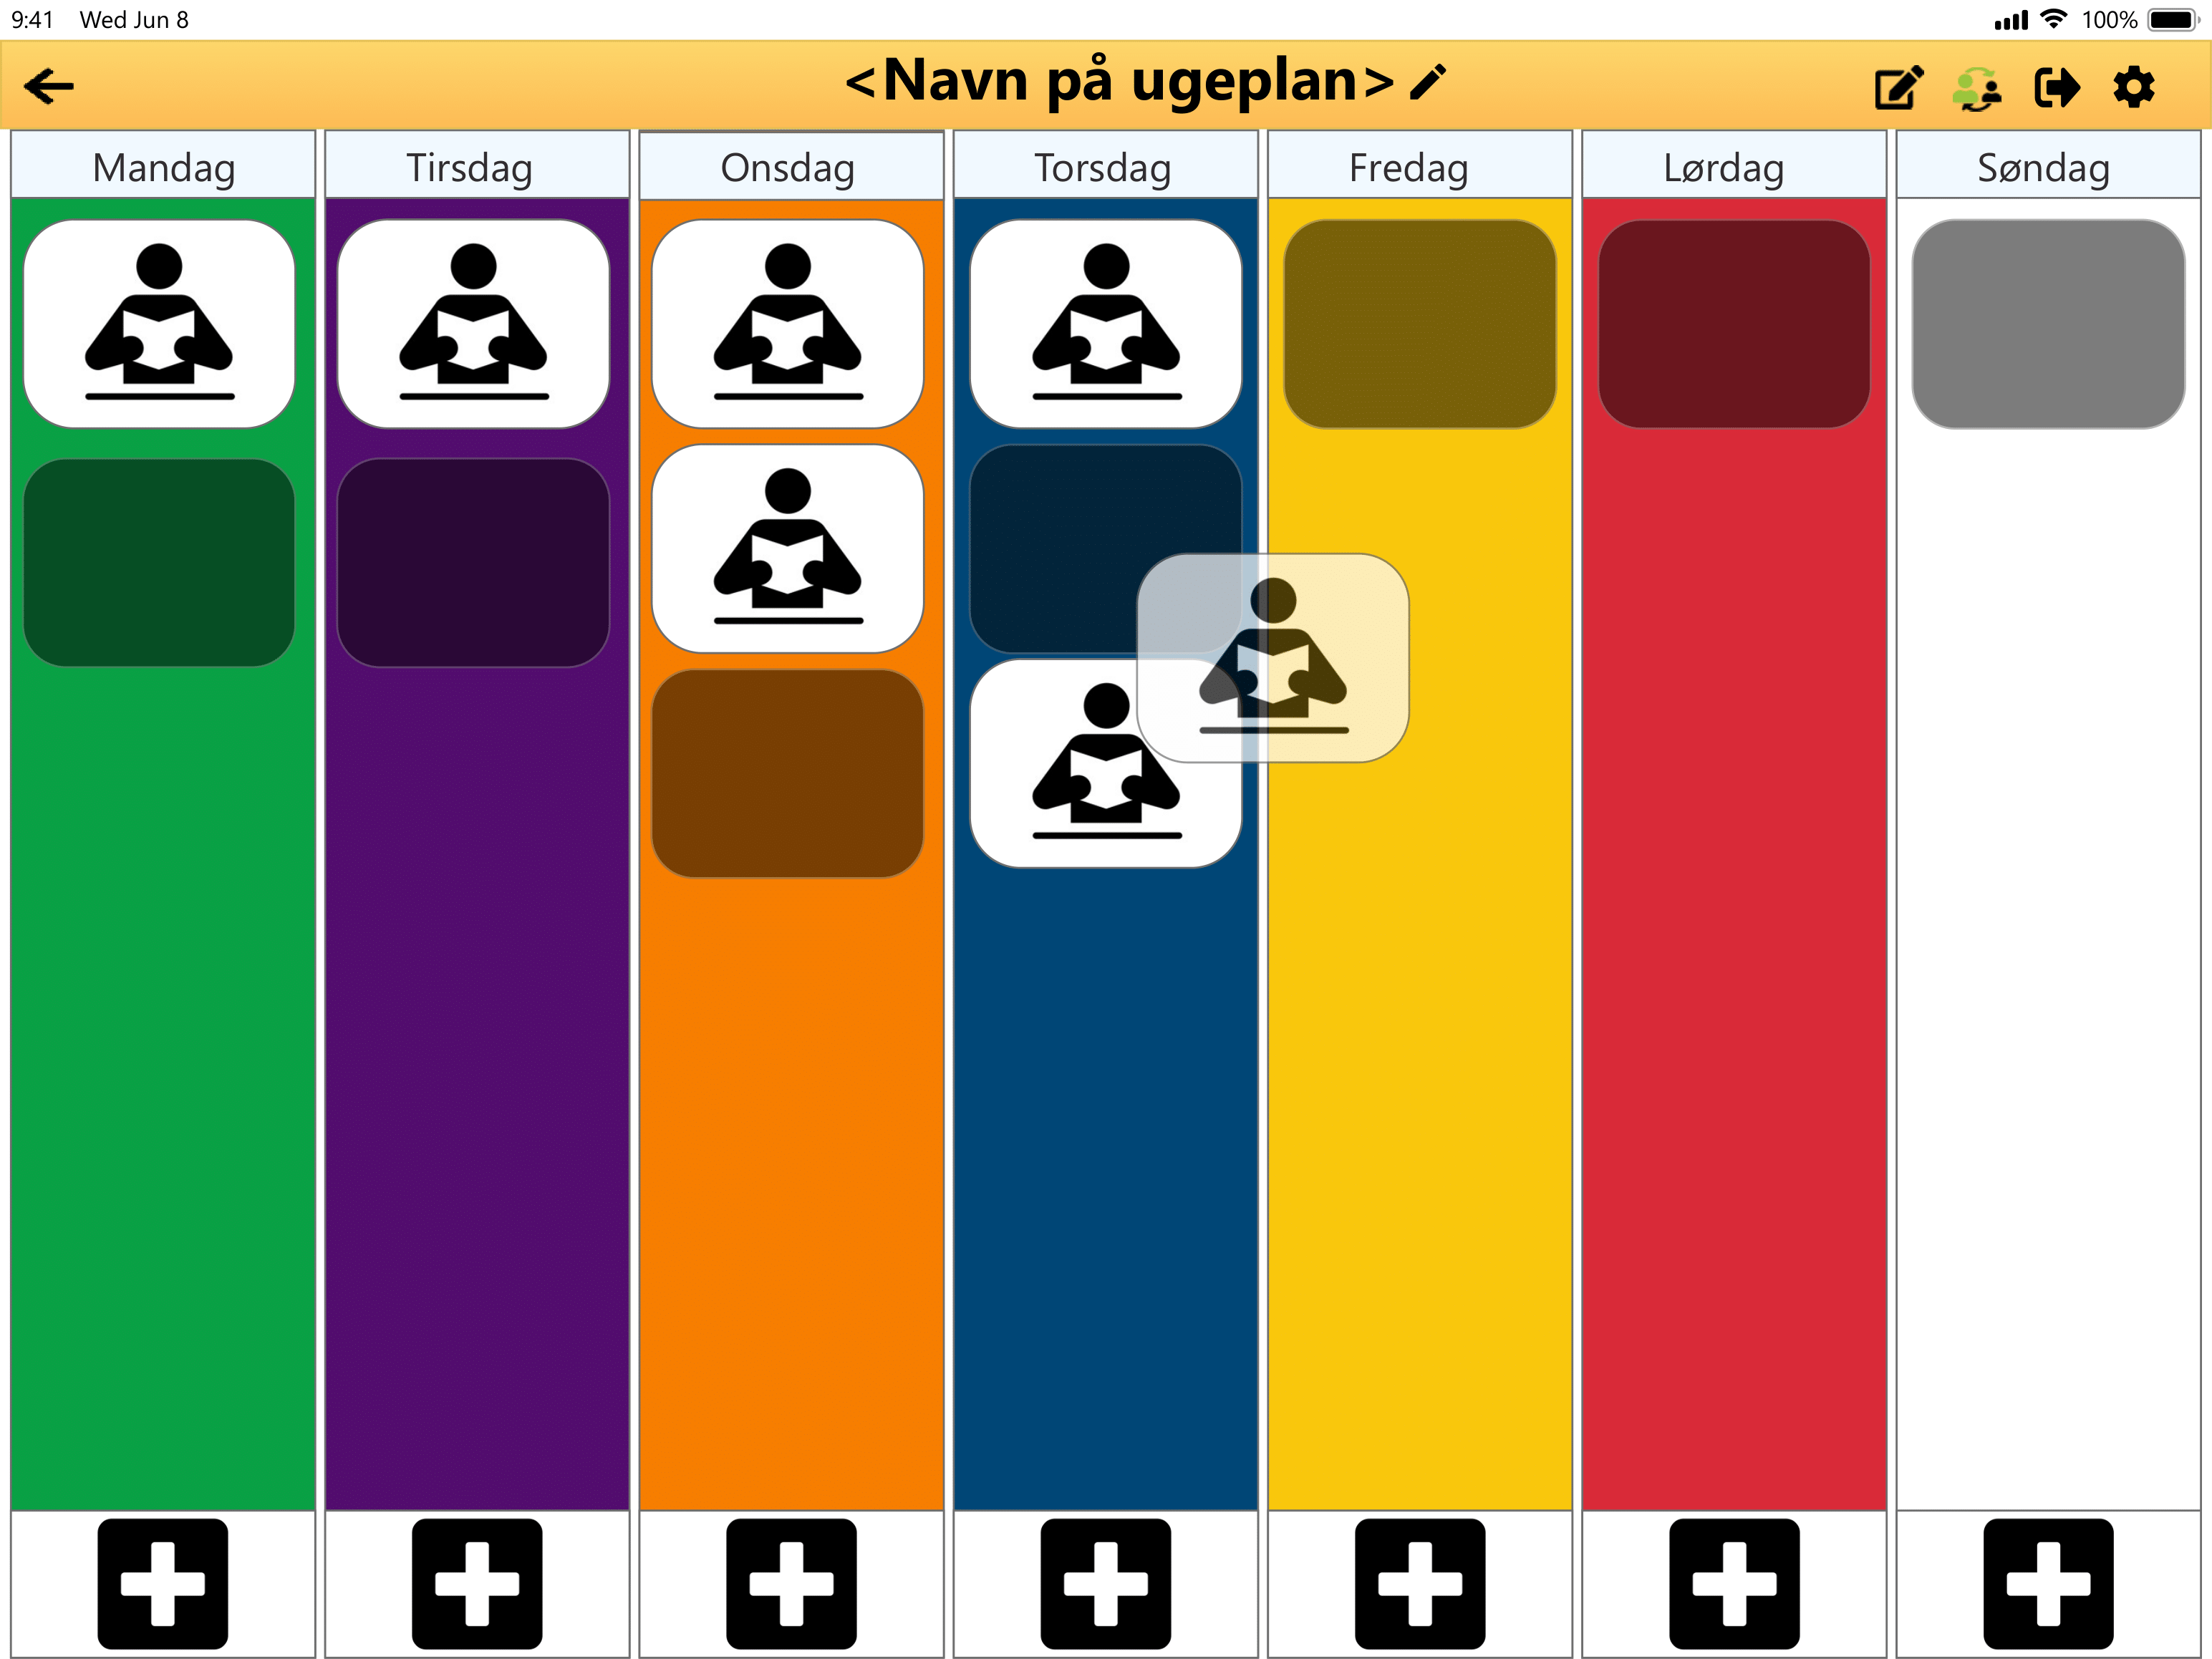
\includegraphics[width=1\linewidth, height=5cm]{drag_n_drop_3.png}
    \caption{Indicatates where activity lands when dropping between activities}
    \label{subfig:drag_n_drop_3}
    \end{subfigure} 
    \caption{}
    \label{fig:drag_n_drop}
\end{figure}

\subsection{Adding citizens}

\begin{figure}[H]
    \begin{subfigure}{0.5\textwidth}
    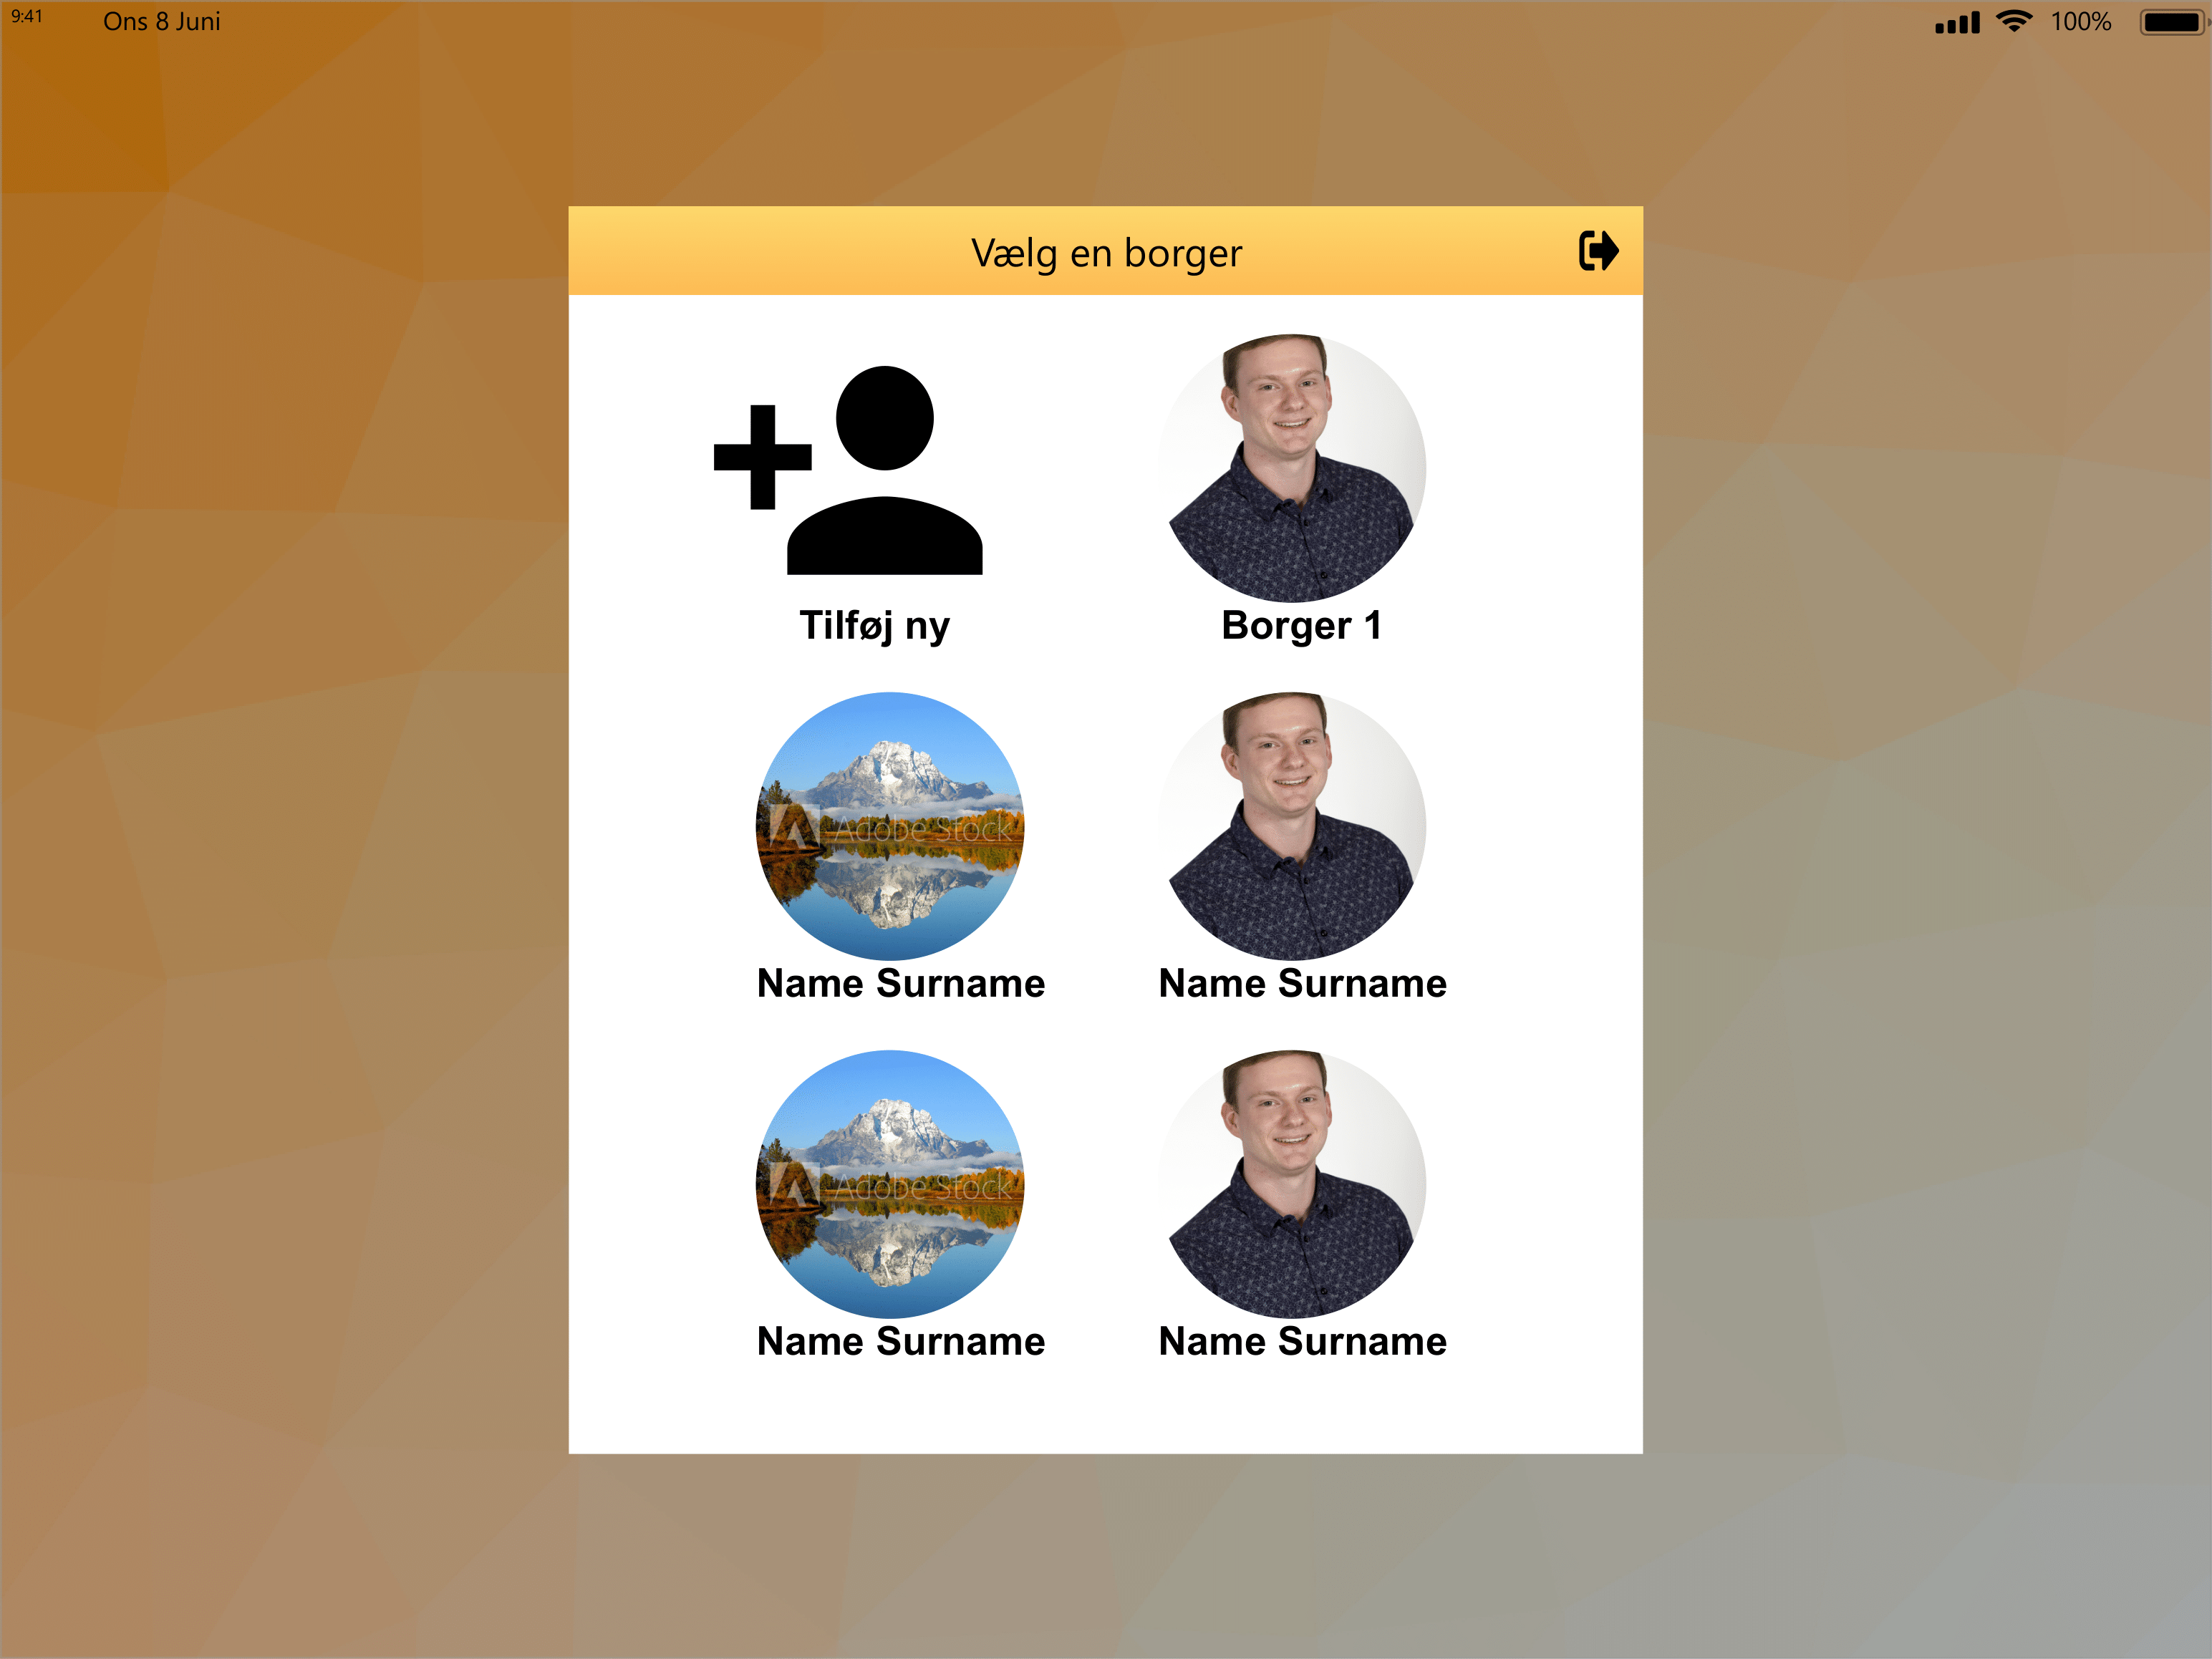
\includegraphics[width=1\linewidth, height=5cm]{add_citizen_1.png}
    \caption{Icon to add new citizen}
    \label{subfig:add_citizen_1}
    \end{subfigure}
    \begin{subfigure}{0.5\textwidth}
        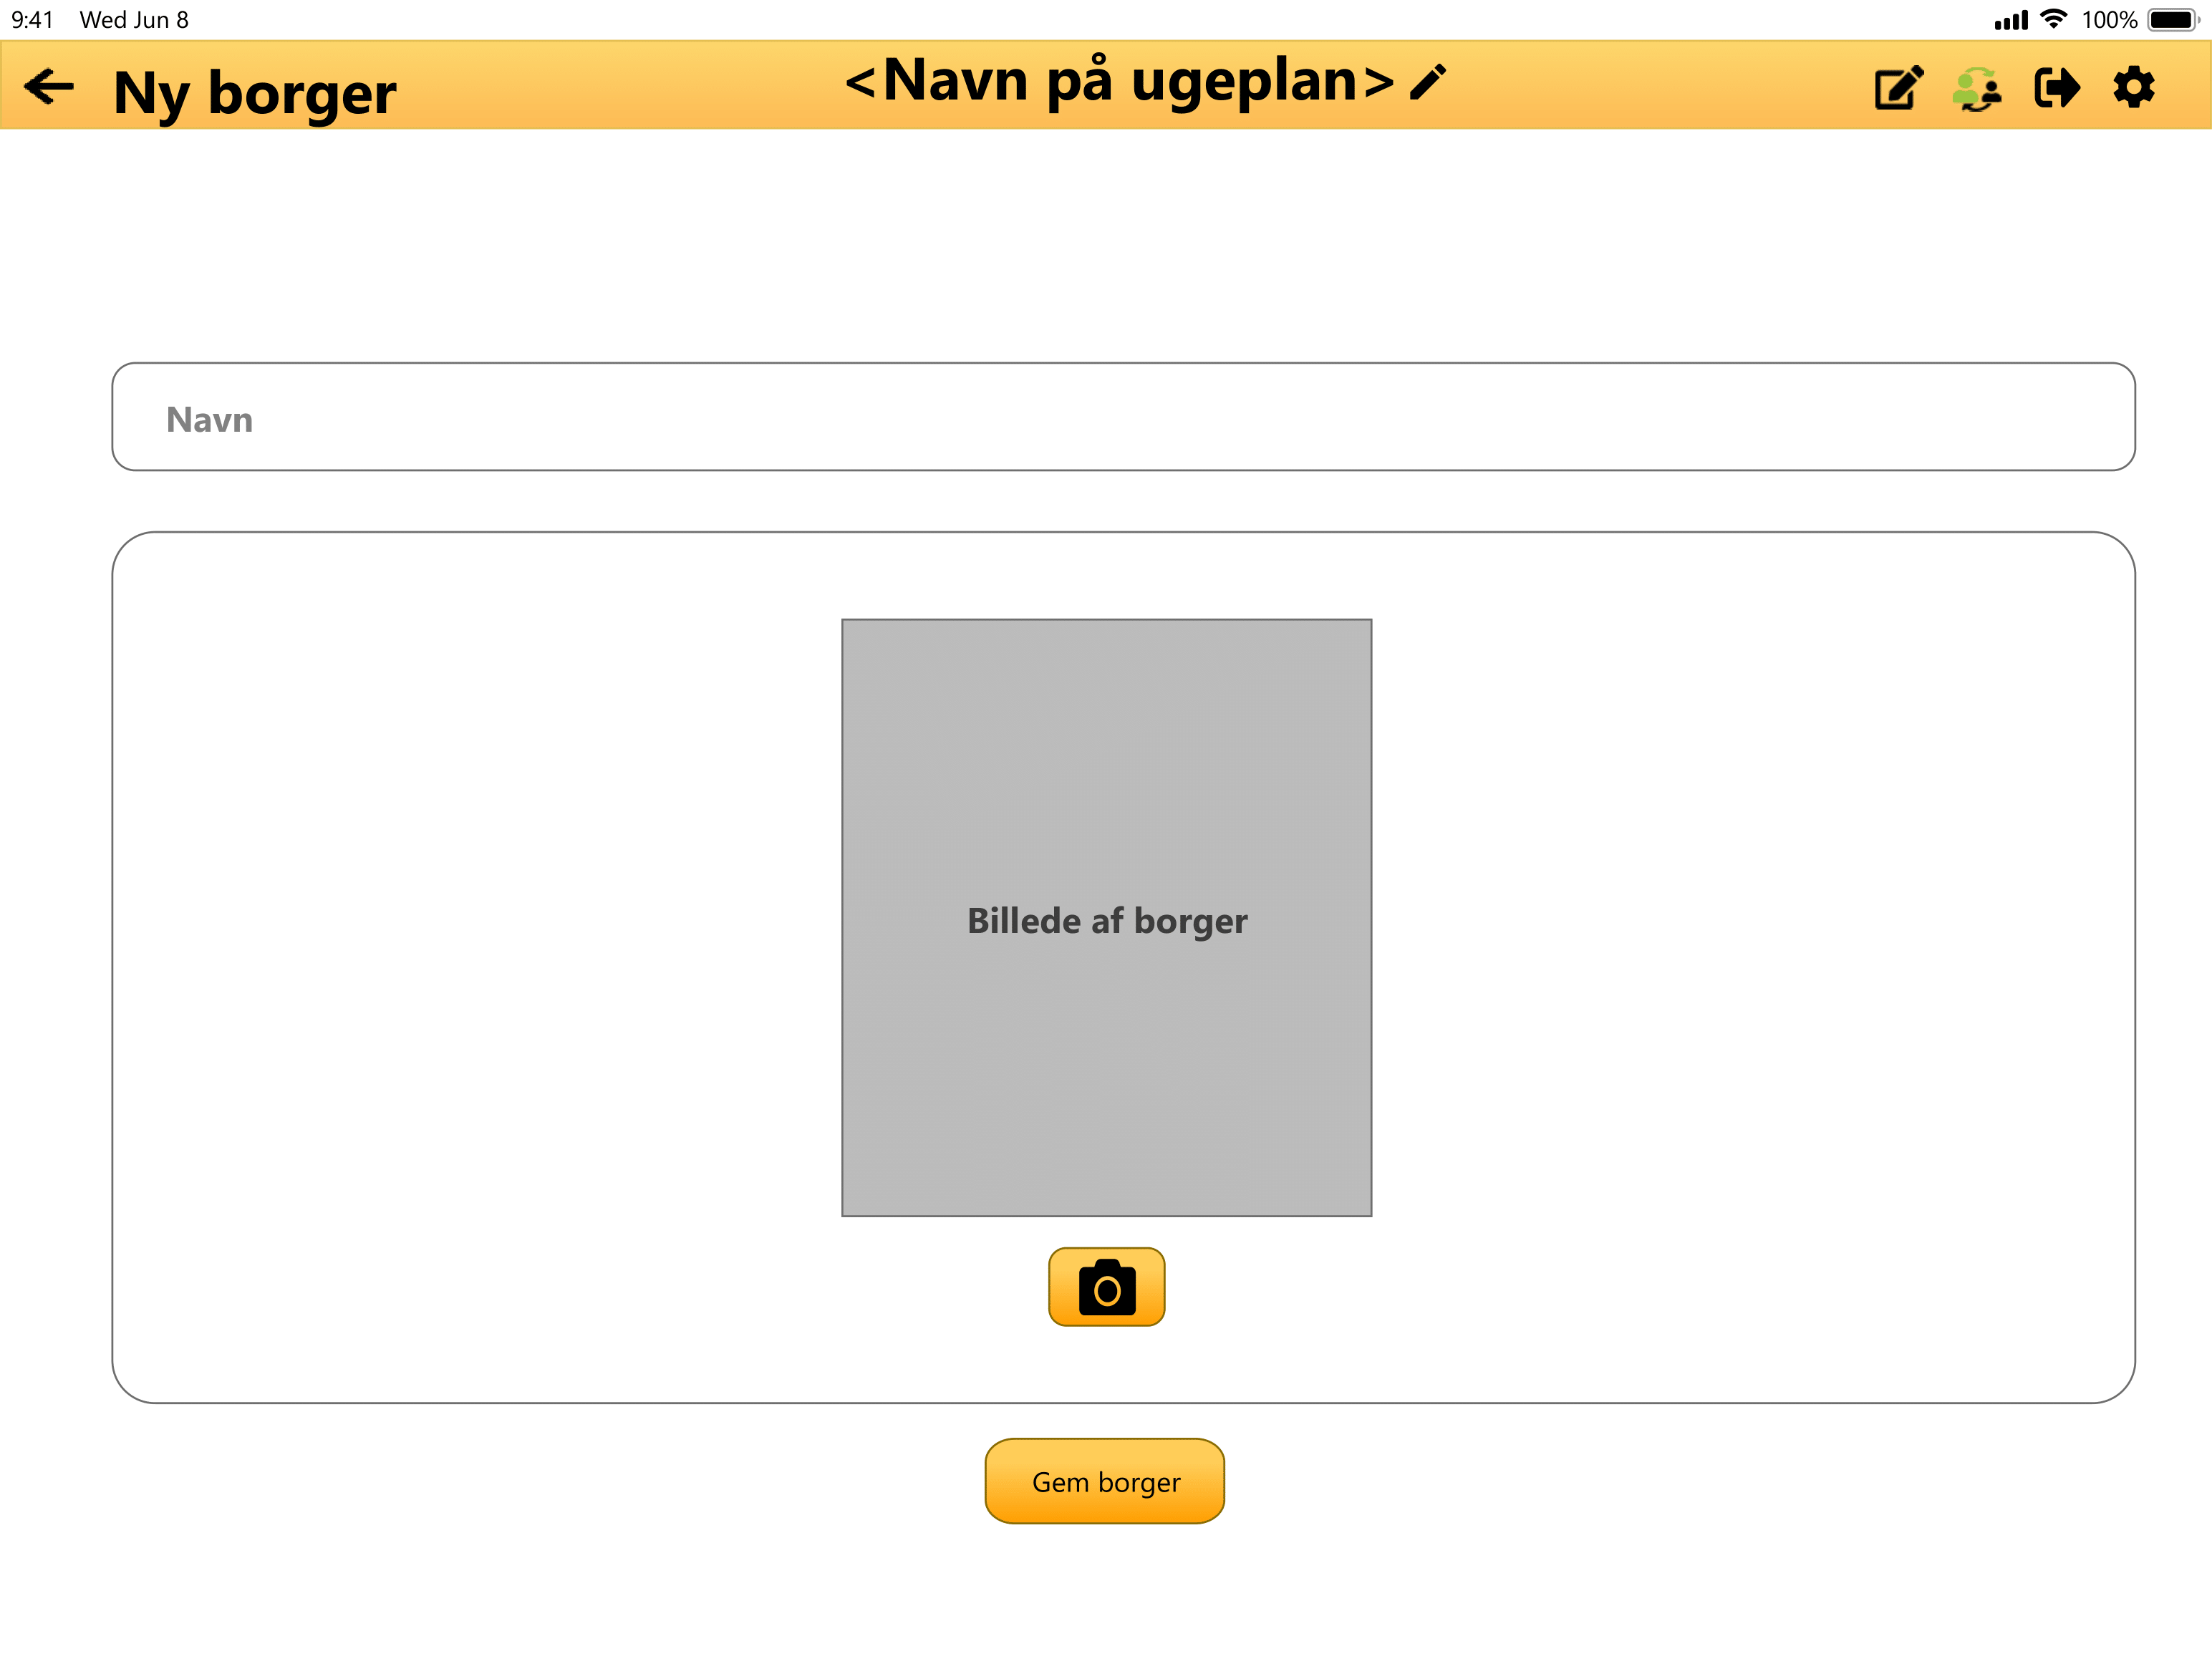
\includegraphics[width=1\linewidth, height=5cm]{add_citizen_2.png}
    \caption{Screen where a new citizen can be created}
    \label{subfig:add_citizen_2}
    \end{subfigure} 
    \caption{}
    \label{fig:add_citizen}
\end{figure}

\subsection{Edit citizens}

\begin{figure}[H]
    \begin{subfigure}{0.5\textwidth}
    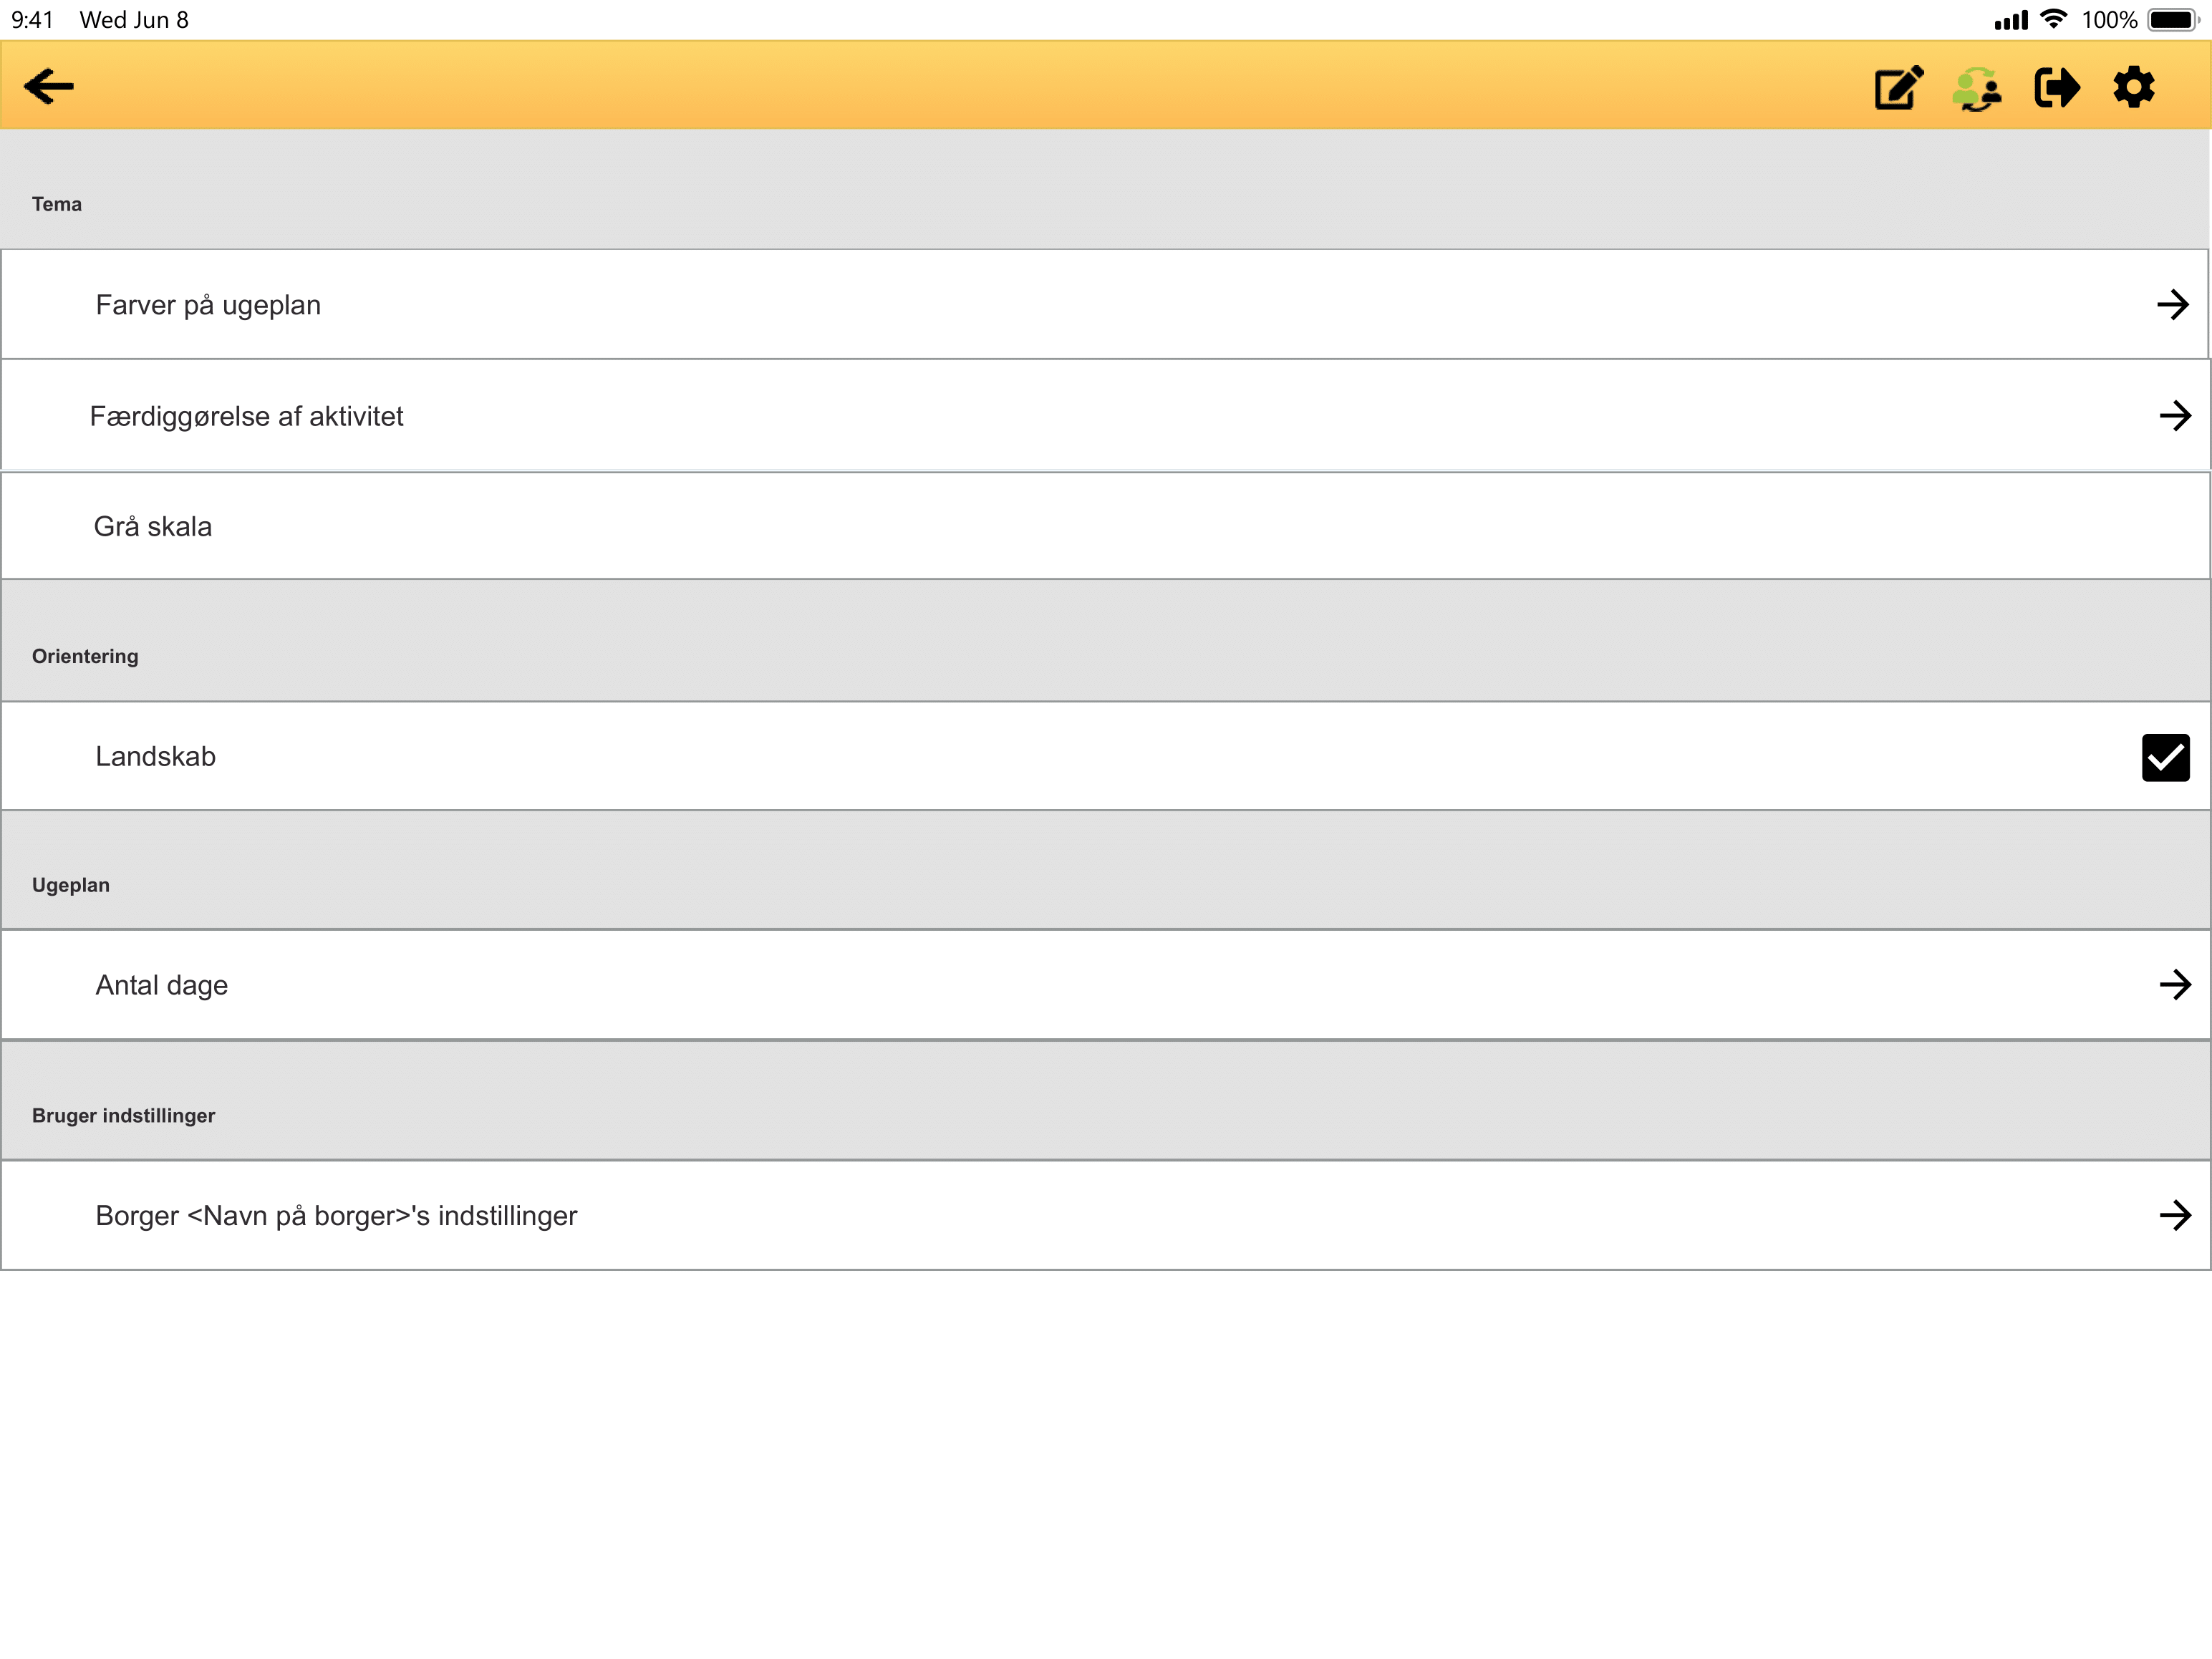
\includegraphics[width=1\linewidth, height=5cm]{edit_citizen_1.png}
    \caption{Settings screen where the guardian can go to the citizens edit screen}
    \label{subfig:edit_citizen_1}
    \end{subfigure}
    \begin{subfigure}{0.5\textwidth}
        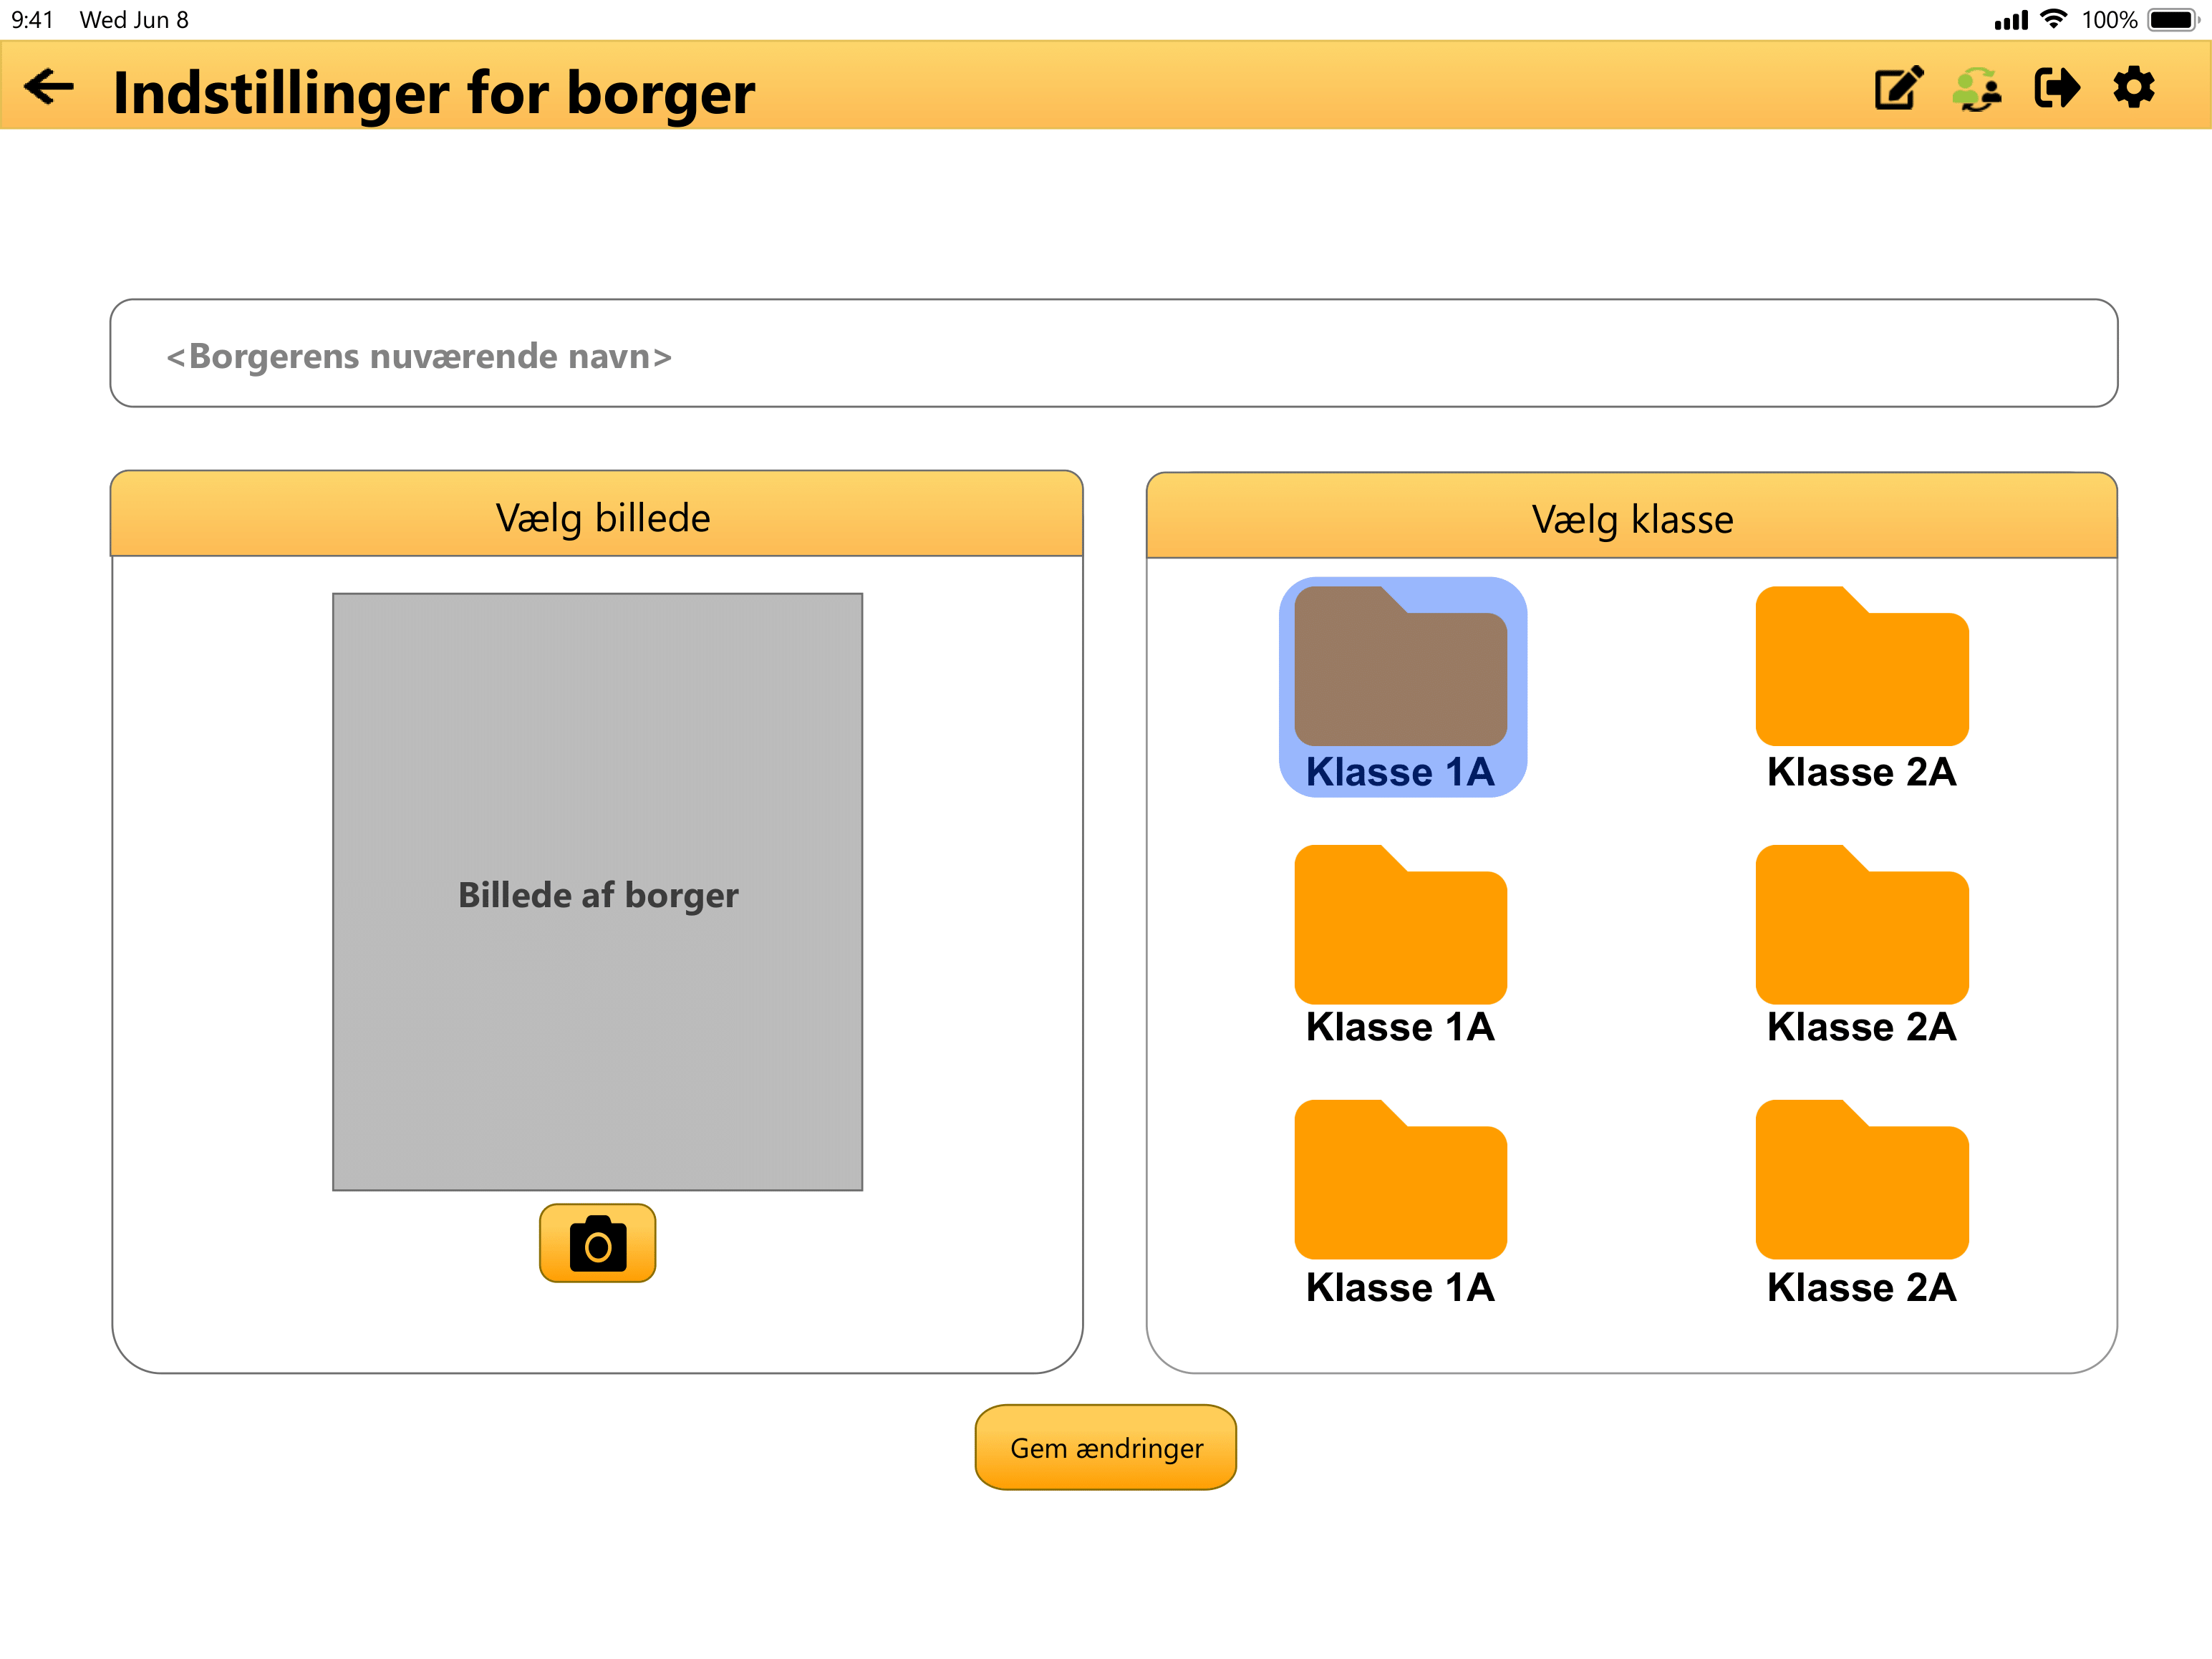
\includegraphics[width=1\linewidth, height=5cm]{edit_citizen_2.png}
    \caption{Edit citizen screen where name, picture and class can be changed}
    \label{subfig:edit_citizen_2}
    \end{subfigure} 
    \caption{}
    \label{fig:edit_citizen}
\end{figure}

\subsection{Deleting week plans}

\begin{figure}[H]
    \begin{subfigure}{0.5\textwidth}
    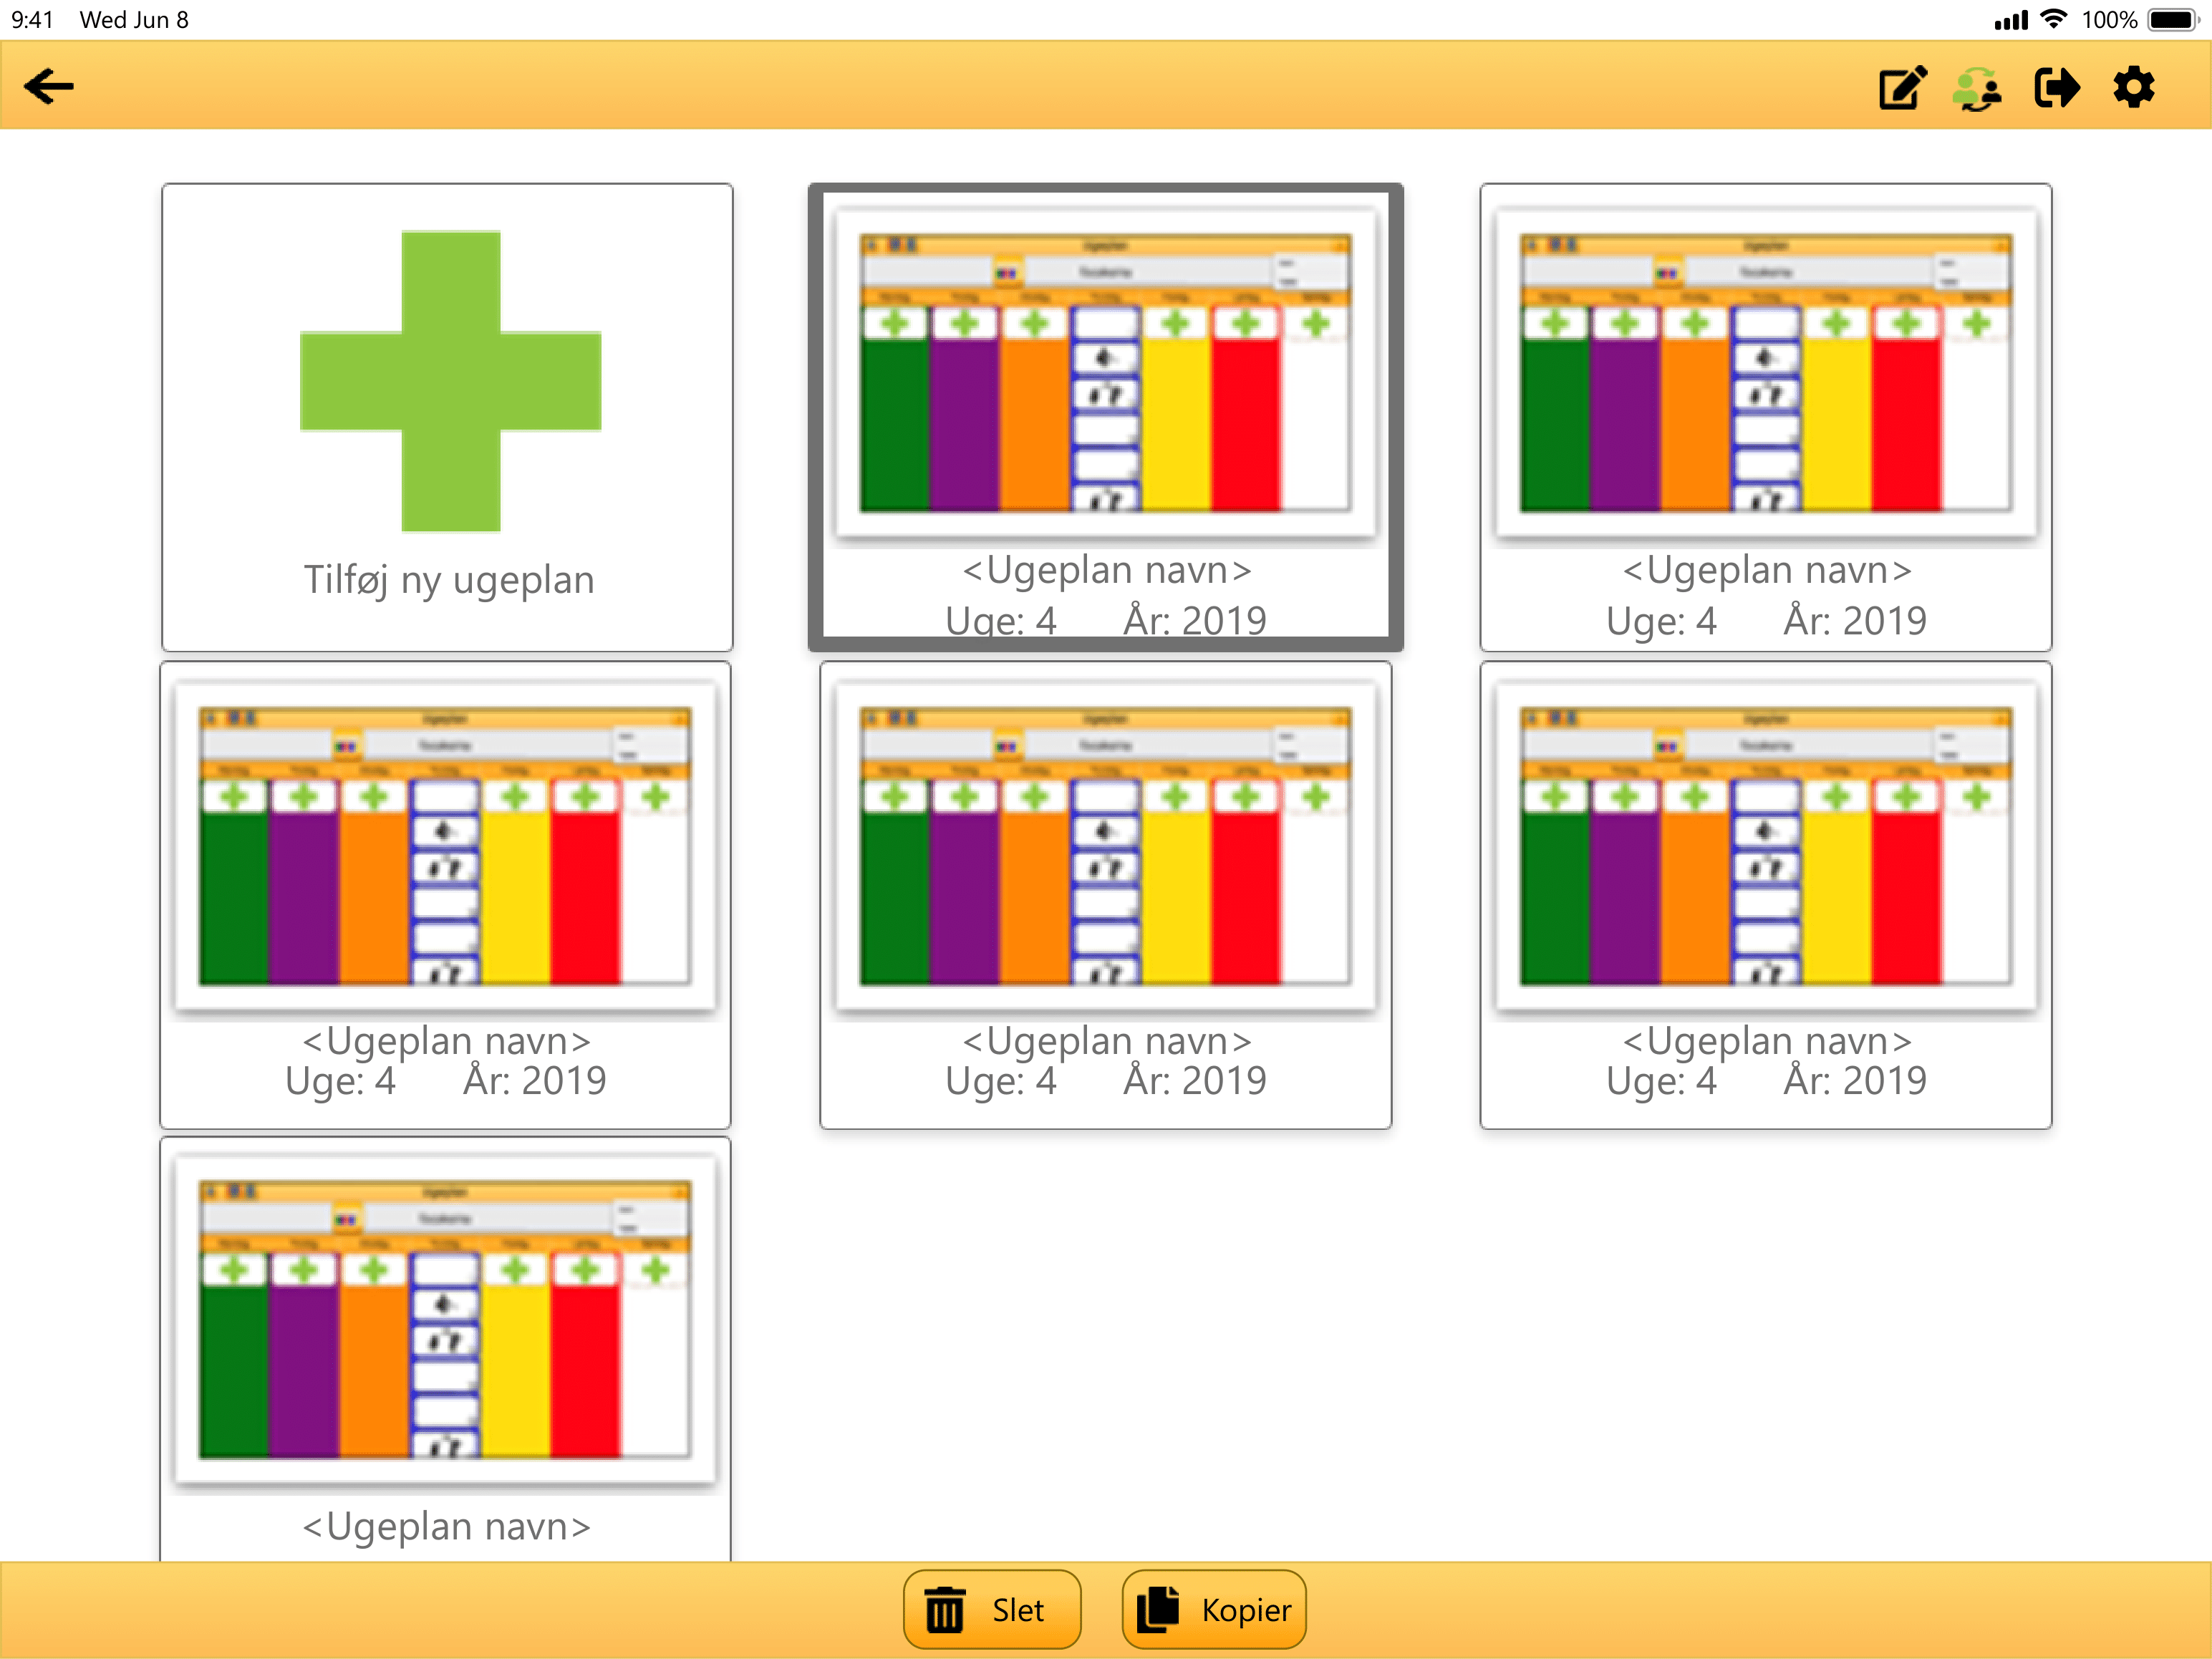
\includegraphics[width=1\linewidth, height=5cm]{delete_weekplan_2.png}
    \caption{Mark week plans through the edit mode}
    \label{subfig:delete_weekplan_2}
    \end{subfigure}
    \begin{subfigure}{0.5\textwidth}
        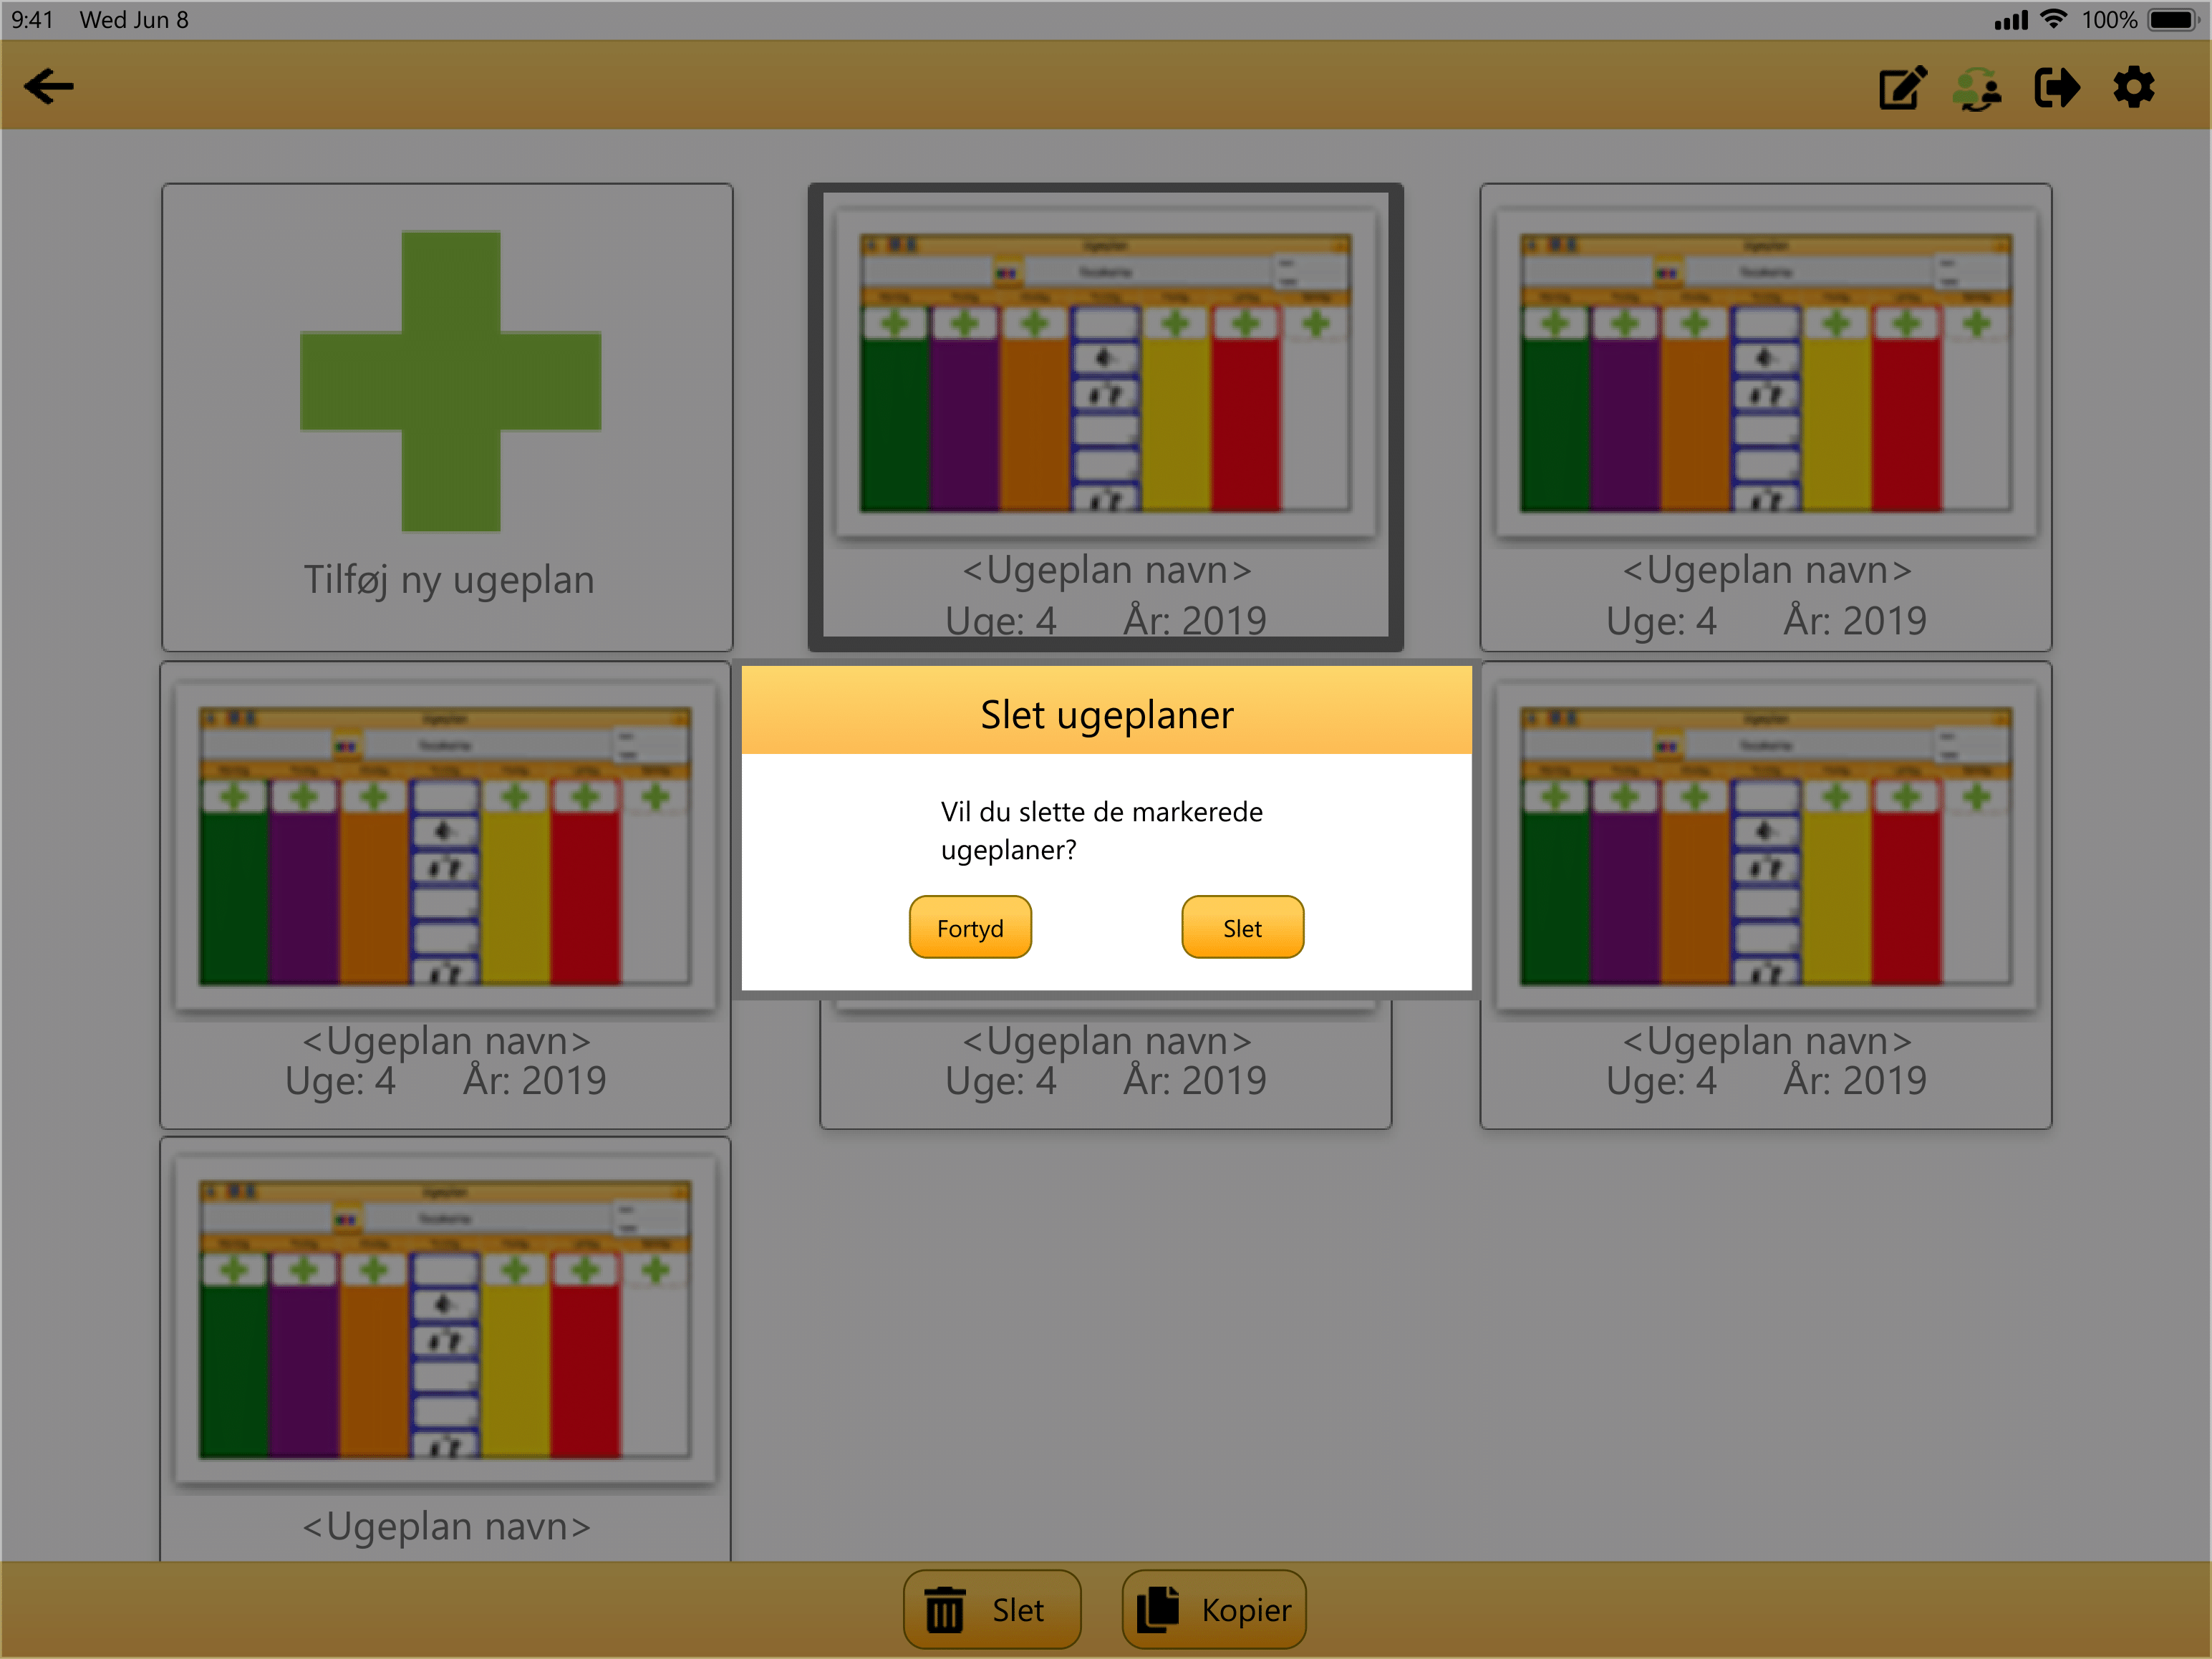
\includegraphics[width=1\linewidth, height=5cm]{delete_weekplan_3.png}
    \caption{Deleting the marked week plans}
    \label{subfig:delete_weekplan_3}
    \end{subfigure} 
    \caption{}
    \label{fig:delete_weekplan}
\end{figure}